% ================================================================
%  第 9 章 Weyl 和与原子能量振荡 (Weyl sums and atomic energy oscillations)
%  依据原书 PDF 第 201--246 页译出；编号审计见文件末尾注释
% ================================================================

\chapter{Weyl 和与原子能量振荡}

\epigraph{元素若按原子量排列，会呈现出性质上明显的周期性.}{Dmitri I. Mendeleev}

\section{目标陈述}

数学家天生是还原论者，常常梦想——也自诩——能够从一小套第一性原理严格推出科学的定律. 这是一个合理的目标，有着辉煌的历史，但极难实现. 而且它很少能打动物理学家，因为数学家能严格证明的东西通常不是他们的热点. 尽管如此，我们总可以引用 E.~Wigner 的评论: 数学作为物理理论表述与发展的基本工具，具有不合理的有效性.

我们从欧几里得那里学到，公理是不证自明的真理；但后来发现——先有 Gauss、Bólyai 与 Lobachevski，后有 Gödel 与连续统假设这个好例子——情况未必总是如此. 另一方面，物理学家常常愿意假设远离自明的新原理，唯一理由是它们极为有用. 薛定谔方程及其波函数解为给定系统的物理性质提供精确描述这一 ansatz 就是如此.

既然这是一本关于调和分析与傅里叶变换的书，似乎应该提及: ``测不准原理''——量子力学的一条基本原理——在好几章中扮演了重要角色: 主要在于这样的陈述: 若光滑函数在构型空间中适应于一个平行多面体（即它在每个方向的导数按平行多面体的相应边长衰减），则其傅里叶变换适应于动量空间中的一个对偶平行多面体，使得两者体积之积必须大于一个绝对常数（滥用语言的话，可以称之为 Planck 常数）. 第 6 章也考虑了通信理论中信号在时间与频率上不能同时受限这一不可能性. 感兴趣的读者可以参阅文献 \cite{b199,b205,b214,b213}，其中展开了傅里叶分析与量子力学中测不准原理的课题.

然而，不多说废话，让我们直接进入正题，声明在本章中我们将研究下面的和，它在非相对论原子能量的渐近分析中起关键作用:
\begin{align*}
  \Psi_{Q}(Z)=\sum_{l=1}^{l_{\mathrm{TF}}}\frac{2l+1}{
  \frac{1}{\pi}\int\bigl(V_{\mathrm{TF}}^{Z}(r)-\frac{l(l+1)}{r^{2}}\bigr)_{+}^{-1/2}\mathrm{d}r}
  \mu\Bigl(\frac{1}{\pi}\int\Bigl(V_{\mathrm{TF}}^{Z}(r)-\frac{l(l+1)}{r^{2}}\Bigr)_{+}^{1/2}\mathrm{d}r\Bigr),
\end{align*}
其中
\begin{align*}
  \mu(x)=\dist\{x,\Z\}^{2}-1/12,
\end{align*}
\begin{itemize}
\item $V_{\mathrm{TF}}^{Z}$ 是电荷为 $Z$ 的 Thomas--Fermi 位势，满足完美的标度条件
\begin{equation}\label{eq:9.1}
  V_{\mathrm{TF}}^{Z}(r)=Z^{4/3}V_{\mathrm{TF}}^{1}(Z^{1/3}r),
\end{equation}
并且有
\begin{equation}\label{eq:9.2}
  V_{\mathrm{TF}}^{1}(r)=\frac{y(ar)}{r},\qquad a=\left(\frac{3\pi}{2}\right)^{2/3},
\end{equation}
其中 $y$ 是 Thomas--Fermi 函数，即 Thomas--Fermi 方程
\begin{equation}\label{eq:9.3}
  \begin{cases}
    y^{\prime\prime}(r)=y^{3/2}(r)/\sqrt{r},\\
    y(0)=1,\\
    \lim_{r\to+\infty}y(r)=0,
  \end{cases}
\end{equation}
的解；

\item $l_{\mathrm{TF}}$ 是使 $V_{\mathrm{TF}}^{Z}(r) - l(l+1)/r^{2}$ 在某处为正的最大整数.
\end{itemize}
这里，记 $(x)_{+}^{-1/2} = x^{-1/2}$（若 $x > 0$），而在其他情形 $(x)_{+}^{-1/2} = 0$.

为理解函数 $\Psi_Q(Z)$ 在原子物理中的作用，让我们简要讨论非相对论分子的 Born--Oppenheimer 模型.

\section{Born--Oppenheimer 模型}

考虑
\begin{itemize}
\item 位于 $y_1, \ldots, y_M \in \R^3$ 的正电荷 $Z_1e, \ldots, Z_Me$ 的 $M$ 个原子核,
\begin{align*}
  Z=(Z_{1},\ldots,Z_{M}),\qquad Y=(y_{1},\ldots,y_{M});
\end{align*}
\item 位于 $x_1, \ldots, x_N \in \R^3$ 的 $N$ 个量子化电子；
\item $e$ = 电子电荷；$m$ = 电子质量；$\hbar$ = Planck 常数.
\end{itemize}
按照 Born--Oppenheimer 模型，非相对论分子由 Hamiltonian
\begin{align*}
  H_{Y,Z,N}=-\sum_{j=1}^{N}\Big(\frac{\hbar}{2m}\Delta_{x_{j}}+\sum_{k=1}^{M}\frac{Z_{k}e^{2}}{\left|x_{j}-y_{k}\right|}\Big)
  +\sum_{1\leq j<k\leq N}\frac{e^{2}}{\left|x_{j}-x_{k}\right|}
  +\sum_{1\leq m<n\leq M}\frac{Z_{n}Z_{m}e^{2}}{\left|y_{n}-y_{m}\right|},
\end{align*}
描述，其中第 $j$ 个 Laplacian 表示第 $j$ 个电子的量子化动能，还有库仑相互作用: 原子核与电子之间的吸引，以及两个排斥项——一个对应原子核之间，另一个对应电子之间.

这个 Hamiltonian 作用于
\begin{align*}
  \mathcal{H}=\bigwedge_{j=1}^{N}L^{2}(\R^{3}\otimes G),\qquad G=\left\{+1,-1\right\}.
\end{align*}
这里，符号 $\wedge$ 表示反对称张量积，编码了 Pauli 不相容原理（电子是满足 Fermi--Dirac 统计的\newterm{fermion}{费米子}{fermion}）；而 $+1$（自旋向上）与 $-1$（自旋向下）表示电子自旋的两种.

\newterm{ground-state-energy}{基态能量}{ground state energy}由
\begin{align*}
  E(Z)=\inf_{N}\inf_{Y}\inf_{\substack{\Psi\in\mathcal{H}\\ \|\Psi\|=1}}\langle\Psi,H_{Y,Z,N}\Psi\rangle
\end{align*}
给出.

要实现用数学解释化学现象的梦想，需要对这些能量作非常精确的计算，而这一任务的难度比今天所能达到的高出好几个量级.

下面，我们将面对更``谦逊''的目标: 迈出解释周期表的第一步，为此只需考虑中性原子的 Hamiltonian 就够了.

\section{中性原子. Hartree--Fock 理论与 Thomas--Fermi 理论}

考虑一个在原点 $y = 0$ 处有 $Z$ 个质子的中性\newterm{atom}{原子}{atom}，并选取单位使 $e^2 = 1$ 且 $\hbar/2m = 1$. 则
\begin{align*}
  H_{Z}=-\sum_{j=1}^{Z}\left(\Delta_{x_{j}}+\frac{Z}{\left|x_{j}\right|}\right)
  +\sum_{1\leq j<k\leq Z}\frac{1}{\left|x_{j}-x_{k}\right|}.
\end{align*}
尽管自旋变量在描述电子行为时是根本的，但从理解数学模型的角度看它们无关紧要. 因此，可以在讨论中省略它们，把态 Hilbert 空间的结构简化为
\begin{align*}
  \mathcal{H}=\bigwedge_{j=1}^{Z}L^{2}(\R^{3})
  =\{\Psi(x_{1},\ldots,x_{Z}),\ x_{j}\in\R^{3}:
  \Psi\in L^{2}(\R^{3Z}),\ \Psi\ \text{反对称}\}.
\end{align*}
反对称意味着对每个置换 $\sigma$，$\Psi(x_{\sigma(1)},\ldots,x_{\sigma(Z)}) = (-1)^{\operatorname{sign}(\sigma)}\Psi(x_1,\ldots,x_Z)$.

电子密度由
\begin{align*}
  \rho(x)=Z\int_{\R^{3(Z-1)}}\left|\Psi(x,x_{2}\ldots,x_{Z})\right|^{2}\,\mathrm{d}x_{2}\cdots\mathrm{d}x_{Z}
\end{align*}
给出，因而
\begin{align*}
  \int_{\Omega}\rho(x)\,\mathrm{d}x
\end{align*}
是 $\Omega \subset \R^3$ 中电子的期望数.

基态能量现在写成
\begin{align*}
  E(Z)=\inf_{\substack{\Psi\in\mathcal{H}\\ \|\Psi\|=1}}\langle\Psi,H_{Z}\Psi\rangle.
\end{align*}
因此，任务在于得到 Hamiltonian $H_{Z}$ 作用于 $3Z$ 维欧氏空间中反对称平方可积函数上的最低特征值. 但这仍然是一个非常困难的问题，主要由于电子的库仑相互作用.

从量子力学的最初年代起，人们就知道显式求解薛定谔方程 $H_{Z}\Psi = \lambda\Psi$ 是不可能的，于是引入了若干近似解法.

若我们的 Hamiltonian 对单电子位势 $V$ 有形如
\begin{align*}
  \widetilde{H}_{Z}=\sum_{k=1}^{Z}\left(-\Delta_{x_{k}}+V(x_{k})\right)
\end{align*}
的形式，则由分离变量，问题将从 $3Z$ 维化归为 $3$ 维. 此外，利用径向对称性，它将变成纯一维（即常微分方程），容易求解.

在量子理论（物理学与化学）中引入的研究原子的主要思想，是用 $\tilde{H}_Z$ 近似 $H_Z$，其中位势 $V(x)$ 选取如下: 让我们暂时假装知道电子密度 $\rho$；那么这样的单电子位势的一个好候选是
\begin{align*}
  V(x)=-\frac{Z}{\left|x\right|}+\int_{\R^{3}}\frac{\rho(y)}{\left|x-y\right|}\,\mathrm{d}y.
\end{align*}
容易推出，$\widetilde{H}_{Z}$ 的基态本征函数与基态电子密度由下面给出:
\begin{itemize}
\item $\Psi_{HF}(x_1,\ldots,x_Z)$，即三维 Schrödinger 算子 $-\Delta + V(x)$ 的本征函数 $\phi_1(x),\ldots,\phi_Z(x)$ 的反对称化乘积（Slater 行列式）；
\begin{align*}
  \rho_{\mathrm{HF}}(x)=\sum_{k=1}^{Z}|\phi_{k}(x)|^{2}.
\end{align*}
\end{itemize}
这一方法（Hartree--Fock）是对原问题的一大简化，因为现在我们面对的只是三维计算而非 $3Z$ 维. 系统通过要求一致性条件（Hartree--Fock 方程）——所得密度等于初始密度——而封闭:
\begin{align*}
  \rho_{\mathrm{HF}}=\rho.
\end{align*}
这是一个引人注目而奇特的方程（既非代数方程、偏微分方程，也非积分方程），通过迭代求解: 从初始密度 $\rho_0$ 出发，产生 Hartree--Fock $\rho_1$；把它作为新的初始数据产生 $\rho_2$，如此继续. 极限密度（假设它存在）将是我们寻求的解.

在这个设定下，容易推出 Hartree--Fock 基态正如上面所指出的，由本征函数的反对称化乘积给出，且负特征值之和是 Hamiltonian 的最低可能能量.

方法是否可行并不显然，无论如何，收敛将依赖于适当初始密度的选取. 在这里，也称原子统计理论的 Thomas--Fermi 理论前来相助，为我们提供三维 Schrödinger 算子的密度与特征值和的良好第一步近似.

Thomas--Fermi 理论是一种用于处理多粒子系统量子力学的技术. 当 $Z$ 很大时，无法指望理解通常的\newterm{wave-function}{波函数}{wave function} $\Psi(x_1, \ldots, x_Z)$. 取而代之，人们试图理解电子密度
\begin{align*}
  \rho(x_{1})=Z\int|\Psi(x_{1},x^{\prime})|^{2}\,\mathrm{d}x^{\prime},
\end{align*}
它是 $x_1 \in \R^3$ 的函数，并希望关于 $\Psi$ 的重要信息都包含在 $\rho = \rho_{\mathrm{TF}}^Z$ 中.

Thomas--Fermi 理论推导出描述 $\rho_{\mathrm{TF}}^{Z}$ 的一个偏微分方程，并从电子密度 $\rho_{\mathrm{TF}}^{Z}$ 的知识猜测系统的能量，见 \cite{b221}. 它把量子力学视为充满相空间、通过库仑排斥与自身相互作用并与位势
\begin{align*}
  V_{\mathrm{TF}}^{Z}(x)=-\frac{Z}{\left|x\right|}+\frac{1}{2}\int_{\R^{3}}\frac{\rho_{\mathrm{TF}}^{Z}(y)}{\left|x-y\right|}\mathrm{d}y
\end{align*}
相互作用的经典气体，该位势满足 \eqref{eq:9.1}--\eqref{eq:9.3} 描述的 Thomas--Fermi 方程；在径向对称性假设下，这些方程变成一个可以求解的非线性常微分方程，表明对参数 $Z$ 的依赖可以通过平凡标度去掉:
\begin{align*}
  \rho_{\mathrm{TF}}^{Z}(x)=Z^{2}\;\rho(Z^{1/3}x),\qquad
  V_{\mathrm{TF}}^{Z}(x)=Z^{4/3}\;V(Z^{1/3}x),
\end{align*}
其中密度 $\rho$ 与位势 $V$ 是完全确定的函数. 这些公式在``原子半径''$Z^{-1/3}$ 与电子间平均距离 $Z^{-2/3}$ 的意义下有自然的解释.

数学中一个成熟悠久的传统是用线性方程近似非线性方程. Thomas--Fermi 与 Hartree--Fock 方法涉及用少数变量的非线性系统近似大量变量的线性系统，见 \cite{b221}.

\begin{remark*}
推导 Thomas--Fermi 方程的关键一步是用电子密度函数表示动能:
\begin{align*}
  \mathcal{E}_{\mathrm{KE}}=C_{\mathrm{TF}}\int\rho^{5/3}(x)\,\mathrm{d}x,
\end{align*}
从而总能量为
\begin{align*}
  \mathcal{E}_{\mathrm{TF}}=C_{\mathrm{TF}}\int\rho^{5/3}(x)\,\mathrm{d}x
  -\int V(x)\rho(x)\,\mathrm{d}x
  +\frac{1}{2}\iint\frac{\rho(x)\rho(y)}{|x-y|}\,\mathrm{d}x\,\mathrm{d}y.
\end{align*}
见 \cite{b221}.
\end{remark*}

为给 Thomas--Fermi 关于 $\mathcal{E}_{\mathrm{KE}}$ 的 ansatz 提供动机，并与第 7 章的格点问题建立有趣的联系，下面我们将描述一个由 $\R^3$ 中 $\delta$-盒 $B_{\delta} = [0, \delta] \times [0, \delta] \times [0, \delta]$ 内 $N$ 个自由粒子组成的玩具模型. 即，假设它们彼此不施力，然后寻找这些粒子所具有的基态能量，它由\newterm{wave-function}{波函数}{wave function} $\Psi(x_1, \ldots, x_N)$ 给出.

注意 $\Psi$ 支于 $B_{\delta} \times \cdots \times B_{\delta} = B_{\delta}^{(N)}$，满足
\begin{align*}
  \int_{B_{\delta}^{(N)}}|\Psi(x_{1},\ldots,x_{N})|^{2}=1,\qquad
  \mathcal{E}_{\mathrm{QE}}=\langle-\Delta\Psi,\Psi\rangle,
\end{align*}
而 $\rho(x_1) = N\int |\Psi(x_1, x')|^2\,\mathrm{d}x'$ 是粒子密度.

再假设\newterm{wave-function}{波函数}{wave function} $\Psi$ 是反对称的（Pauli 不相容原理），然后求能量最小的态，即基态.

设 $f_1, f_2, \ldots$ 是 $-\Delta$ 在 $B_\delta$ 中 Dirichlet 边界条件下的本征函数，$\lambda_1, \lambda_2, \ldots$ 是相应的特征值. 由于 $\R^{3N}$ 中的 Laplacian 经分离变量分裂，我们问题的本征函数将是
\begin{align*}
  \Psi_{m_{1},\ldots,m_{N}}(x_{1},\ldots,x_{N})=f_{m_{1}}(x_{1})\cdots f_{m_{N}}(x_{N}),
\end{align*}
特征值为 $\lambda_{m_1} + \cdots + \lambda_{m_N}$.

考虑到反对称性，若希望 $\Psi$ 不恒等于零，必须选取不同的 $m_j$. 于是得到反对称本征函数
\begin{align*}
  \Psi_{m_{1},\ldots,m_{N}}(x_{1},\ldots,x_{N})
  =\frac{1}{N!}\sum_{\sigma\in S_{N}}\operatorname{sign}(\sigma)f_{m_{1}}(x_{1})\cdots f_{m_{N}}(x_{N}),
\end{align*}
其中和对对称群 $S_{N}$ 的所有元素 $\sigma$ 进行.

但我们在盒 $B_{\delta}$ 中显式地知道这些本征函数；它们是
\begin{align*}
  \prod_{j=1}^{3}\sin\Bigl(\frac{\pi\nu_{j}\cdot x_{j}}{\delta}\Bigr),\qquad
  \nu_{j}=(\nu_{j}^{1},\nu_{j}^{2},\nu_{j}^{3})\in\Z^{3},
\end{align*}
相应的特征值是
\begin{align*}
  \frac{\pi^{2}}{\delta^{2}}\left((\nu_{j}^{1})^{2}+(\nu_{j}^{2})^{2}+(\nu_{j}^{3})^{2}\right)
  =\frac{\pi^{2}}{\delta^{2}}|\nu_{j}|^{2}.
\end{align*}
为估计前几个特征值之和，取一个包含 $N$ 个格点（也许除小误差外）的半径 $r$ 的球，并注意
\begin{align*}
  N\simeq\operatorname{vol}\{|\xi|<r:\xi_{j}\geq 0\}\simeq r^{3}.
\end{align*}
因此，能量为
\begin{align*}
  \simeq\int_{|\xi|<r,\ \xi_{j}>0}\frac{\pi^{2}}{\delta^{2}}|\xi|^{2}\,\mathrm{d}\xi=C\frac{r^{5}}{\delta^{2}},
\end{align*}
把它写成
\begin{align*}
  C\left(\frac{N}{\delta^{3}}\right)^{5/3}\delta^{3}.
\end{align*}
但 $N/\delta^{3}$ 是盒 $B_{\delta}$ 中的粒子密度，$\delta^{3}$ 是体积. 因此，把空间分成小盒 $B_{\delta}^{k}$——其中 $\rho = \rho_{k}$ 近似为常数——把所有上述项相加，并在粒子数 $N$ 足够大时取极限，就得到所寻求的动能表达式
\begin{align*}
  C_{\mathrm{TF}}\int\rho^{5/3}(x)\,\mathrm{d}x.
\end{align*}
该公式的精确推导以及 Hartree--Fock 方程更易处理的形式，见 \cite{b221,b220}.

\section{原子的基态能量}

上面的文字只是呈现此处要点所需的 Hartree--Fock 与 Thomas--Fermi 理论的粗略印象式概述；要点是对原子基态能量的严格（数学定理）结果，它可以总结为下面的（渐近）展开:
\begin{align*}
  E(Z)=C_{\mathrm{TF}}Z^{7/3}+C_{\mathrm{s}}Z^{2}+C_{\mathrm{sd}}Z^{5/3}+\Psi_{Q}(Z)+\cdots.
\end{align*}
\begin{itemize}
\item 项 $C_{\mathrm{TF}}Z^{7/3}$ 于 1927 年由 Thomas--Fermi \cite{b212,b226} 提出，于 1977 年由 Lieb--Simon \cite{b221} 证明.
\item 项 $C_sZ^2$ 首先出现在数值计算中，于 1952 年由 Scott \cite{b222} 解释，并由 Hughes--Siedentop--Weikard 于 1985--89 年 \cite{b224,b225,b218} 严格证明. 它反映了靠近原子核的电子行为仿佛没有电子相互作用（屏蔽效应）.
\item 项 $C_{\mathrm{SD}}Z^{5/3}$ 于 1930 年由 Dirac \cite{b203}、1981 年由 Schwinger \cite{b223} 猜想. 它于 1990 年由 Fefferman--Seco \cite{b207} 证明. 它代表由微妙的电子关联引起的小效应.
\end{itemize}
下一项 $\Psi_Q(Z)$ 是振荡的，由前面陈述过的公式给出:
\begin{align*}
  \Psi_{Q}(Z)=\sum_{l=1}^{l_{\mathrm{tr}}}\frac{2l+1}{
  \frac{1}{\pi}\int\mathcal{F}(r)^{-1/2}\,\mathrm{d}r}
  \cdot\mu\Bigl(\frac{1}{\pi}\int\mathcal{F}(r)^{1/2}\,\mathrm{d}r\Bigr),
\end{align*}
其中
\begin{align*}
  \mathcal{F}(r):=\left(V_{\mathrm{TF}}^{Z}(r)-\frac{l(l+1)}{r^{2}}\right)_{+},
\end{align*}
约定 $x \leq 0$ 时 $(x)_{+} = 0$，其中
\begin{align*}
  V_{\mathrm{TF}}^{Z}(r)=Z^{4/3}V(Z^{1/3}r)
\end{align*}
是 Thomas--Fermi 位势，而
\begin{align*}
  l_{\mathrm{TF}} = \{\text{使 } V_{\mathrm{TF}}^{Z}(r) - l(l + 1)/r^{2} > 0 \text{ 在某处成立的最大整数 } l\}.
\end{align*}
最后,
\begin{align*}
  \mu(x)=\dist(x,\Z)^{2}-\frac{1}{12}.
\end{align*}
$\mu(x)$ 的图象如下所示.

\begin{center}
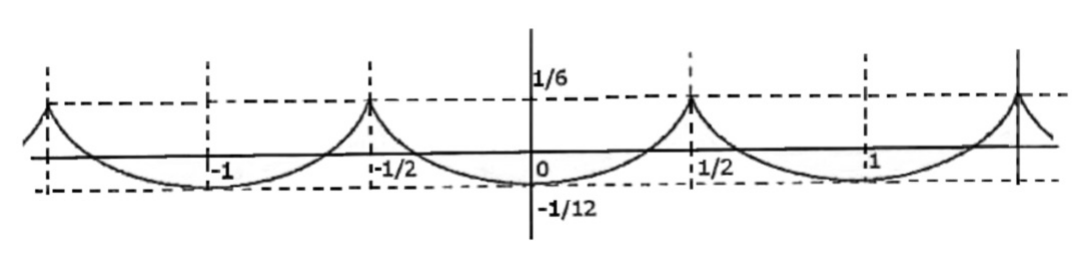
\includegraphics[width=0.6\textwidth]{figs/fig-9-energy.png}
\end{center}

$\Psi_Q$ 的振荡（殆周期的）特征非常有趣，有相当的理由相信它编码了价电子对能量的贡献. 我们对这一项的分析包含在下面的定理中.

\begin{theorem}\label{thm:9.1}
\begin{align*}
  -c_{1}Z^{3/2}\leq\Psi_{Q}(Z)\leq c_{1}Z^{3/2},\qquad
  \Bigl(\frac{1}{Z}\int_{1}^{Z}|\Psi_{Q}(u)|^{2}\,\mathrm{d}u\Bigr)^{1/2}\geq c_{2}Z^{3/2},
\end{align*}
其中 $0 < c_1, c_2 < \infty$ 是普适常数.
\end{theorem}

特别地，有
\begin{align*}
  |\Psi_{Q}| \text{ 的平均} \approx Z^{3/2}.
\end{align*}

本章其余部分将致力于给出定理 9.1 证明的细节. 这是一个冗长的论证，涉及一系列类似的振荡积分计算，采用驻相法、van der Corput 估计与泊松求和公式等技术. 在某种意义上，如引言中所指出的，它位于第 1 章数学俳句的对跖点.

对精通原子数学理论、熟悉文献 \cite{b208,b209,b218,b221} 内容的读者，本章将提供对基态能量渐近展开中这个引人入胜的振荡项的估计的全面阐述. 然而，对那些不熟悉 Hartree--Fock 与 Thomas--Fermi 模型、但对前面各章的调和分析感兴趣的读者，深入这个证明的细节可以进一步坚定他们对这一领域作为描述自然现象的合适工具之力量的信念. 还可以认为，它作为激励去探索上述文献中丰富而有力的数学，并且也许将促进数学梦想中``以几何方式证明''（more geometrico demonstrata）化学的进展，正如 Spinoza 会说的那样.

在我们的分析中，首先解码它的表达式，强调它与数论中一些经典公式的类比，即欧氏空间区域内数格点问题中出现的那些公式. 然后我们可以利用数论学家为处理三角和而引入的工具来完成定理的证明.

从抽象数学的角度看，诸如 $\Psi_Q$ 的和相当古老，最著名的可上溯至 Gauss，它与估计凸区域内整格点数有关，如第 7 章所考虑的.

值得注意我们的问题与圆问题之间的密切相似性，后者来自对盒中量子自由粒子束缚态数目的精细分析.

证明组织如下. 首先，在对众所周知的驻相引理作一些平凡修改之后（9.5 节），我们（在 9.6 节）着手研究形如
\begin{align*}
  S(\lambda)=\sum_{l=1}^{\lambda}f\Big(\frac{l}{\lambda}\Big)\mu\Big(\lambda\phi\Big(\frac{l}{\lambda}\Big)\Big)
\end{align*}
的和，其中 $\phi''(x) \geq c_0 > 0$，$\mu$ 是平均为 $0$ 的周期函数. 这类和的例子如下.

\begin{enumerate}
\item 若 $f \equiv 1$，$\mu(x) = e^{2\pi ix}$，$\phi(x) = x^2$，则得到模 $\lambda$ 的著名 Gauss 和.
\item 若 $f \equiv 1$，$\mu(x) = x - [x] - 1/2$，则 $S$ 表示被 $\lambda$ 膨胀的曲线 $\phi$ 的格点问题中的误差项.
\end{enumerate}

虽然上面第一项已被充分理解，第二项仍然非常困难. 在我们的情形中，只需处理傅里叶系数衰减相当快（$\hat{\mu}(n) \sim |n|^{-3/2+\varepsilon}$）的函数 $\mu$，这允许用 van der Corput 的通常方法（泊松求和接驻相法；见 \cite{b215}）对这些和作完全分析，因为所有表达式都绝对收敛. 这里还需要一点初等数论论证来排除小分母问题的可能性，它产生一个大小依赖于某个数是有理数还是无理数的误差项.

在 9.7 节中，我们把 9.6 节的结果应用于 $\Psi_Q$，得到一个新的和 $\Psi_0$，即 $\Psi_Q$ 的领头``对偶''版本，令人想起模函数的 Jacobi 恒等式. $\Psi_Q$ 的精确上界是它的容易推论. 然而，为得到 $\Psi_Q$ 公式中所涉曲线与振幅的正确正则性性质，结果相当繁琐.

在 9.8 节中，通过理解 $\Psi_0$ 在平均意义下的行为，我们以 $\Omega$-结果的形式得到 $\Psi_Q$ 的下界.

这些结果最初发表于 \cite{b200,b201}，以下数页几乎是这些论文内容的逐字转录，它们严重依赖 \cite{b208} 中证明的估计.

\section{驻相估计}

让我们从回顾驻相开始. 考虑 $f \in C_0^\infty(\R)$. 则若 $t > 0$,
\begin{align*}
  \int_{-\infty}^{\infty}e^{i t x^{2}}f(x)\,\mathrm{d}x
  =e^{\pi i/4}\sqrt{\frac{\pi}{t}}\int_{-\infty}^{\infty}e^{-\pi^{2}i\xi^{2}/t}\widehat{f}(\xi)\,\mathrm{d}\xi.
\end{align*}
利用恒等式
\begin{align*}
  e^{s}=1+\int_{0}^{1}e^{su}s\,\mathrm{d}u,
\end{align*}
推出
\begin{equation}\label{eq:9.4}
  \begin{aligned}
  \int_{-\infty}^{\infty}e^{itx^{2}}f(x)\,\mathrm{d}x
  &=e^{\pi i/4}\sqrt{\frac{\pi}{t}}\left(f(0)+\int_{-\infty}^{\infty}\widehat{f}(\xi)
   \int_{0}^{1}\frac{-\pi^{2}i\xi^{2}}{t}e^{-\pi^{2}iu\xi^{2}/t}\,\mathrm{d}u\,\mathrm{d}\xi\right)\\
  &=e^{\pi i/4}\sqrt{\frac{\pi}{t}}\left(f(0)+\frac{i}{4t}\int_{-\infty}^{\infty}\widehat{f^{\prime\prime}}(\xi)
   \int_{0}^{1}e^{-\pi^{2}iu\xi^{2}/t}\,\mathrm{d}u\,\mathrm{d}\xi\right)\\
  &=e^{\pi i/4}\sqrt{\frac{\pi}{t}}f(0)+\frac{i}{4t}\int_{-\infty}^{\infty}f^{\prime\prime}(x)
   \int_{0}^{1}e^{itx^{2}/u}\frac{\mathrm{d}u}{u^{1/2}}\,\mathrm{d}x\\
  &=e^{\pi i/4}\sqrt{\frac{\pi}{t}}f(0)+\frac{i}{4t^{3/2}}\int_{-\infty}^{\infty}f^{\prime\prime}(x)g_{t}(x)\,\mathrm{d}x,
  \end{aligned}
\end{equation}
其中
\begin{align*}
  g_{t}(x)=\int_{0}^{1}e^{itx^{2}/u}\left(\frac{t}{u}\right)^{1/2}\mathrm{d}u.
\end{align*}
注意 $g_{t}(x)=t^{1/2}g_{1}(t^{1/2}x)$，且
\begin{align*}
  g_{1}(x)=i\,e^{i x^{2}/u}\frac{u^{3/2}}{x^{2}}\Big|_{0}^{1}-\frac{3i}{2}\int_{0}^{1}e^{i x^{2}/u}\frac{u^{1/2}}{x^{2}}\,\mathrm{d}u,
\end{align*}
因此 $|g_1(x)| \leq 2/|x|^2$，从而 $g_1$ 可积. 此外,
\begin{align*}
  \|g_{t}\|_{1}=\|g_{1}\|_{1}=O(1),\qquad
  |g_{t}(x)|\leq 2|x|^{-2}t^{-1/2}.
\end{align*}
我们还考虑形如
\begin{align*}
  \int_{0}^{\infty}e^{itx^{2}}f(x)\,\mathrm{d}x
\end{align*}
的单侧积分. 定义
\begin{align*}
  f^{+}(x)=\begin{cases}
    f(x), & \text{若 } x\geq 0,\\
    f(-x), & \text{若 } x\leq 0,
  \end{cases}
\end{align*}
并考虑 $f_{\varepsilon} = f^{+} * \varphi_{\varepsilon}$，其中 $\varphi_{\varepsilon}$ 是恒等算子的适当逼近. 用我们之前的恒等式，得
\begin{align*}
  &\int_{0}^{\infty}e^{itx^{2}}f(x)\,\mathrm{d}x\\
  &=\frac{1}{2}\lim_{\varepsilon\rightarrow 0}\int_{-\infty}^{\infty}e^{itx^{2}}f_{\varepsilon}(x)\,\mathrm{d}x
  =\frac{1}{2}e^{\pi i/4}\sqrt{\frac{\pi}{t}}f(0)
   +\frac{i}{8t^{3/2}}\lim_{\varepsilon\rightarrow 0}\int_{-\infty}^{\infty}f_{\varepsilon}^{\prime\prime}(x)g_{t}(x)\,\mathrm{d}x\\
  &=\frac{1}{2}e^{\pi i/4}\sqrt{\frac{\pi}{t}}f(0)
   +\frac{i}{4t^{3/2}}\int_{0}^{\infty}f^{\prime\prime}(x)g_{t}(x)\,\mathrm{d}x.
\end{align*}
最后一步成立是因为 $g_{t}$ 可积，且函数 $g_{t}$ 与 $f^{+}$ 都为偶.

\begin{definition}\label{def:9.2}
设 $\phi$ 满足
\begin{align*}
  |\phi^{(n)}(x)|\leq C_{n}\quad (0\leq n\leq 5),\qquad
  c_{0}=\inf|\phi^{\prime\prime}(x)|>0,
\end{align*}
对某个在应用中会明确的区间中的 $x$ 成立. 记
\begin{align*}
  c_{0}^{+}=\min\{1,c_{0}\},\qquad
  B(\phi)=\left(\frac{1+\|\phi\|_{C^{5}}}{c_{0}^{+}}\right)^{54}.
\end{align*}
\end{definition}

\begin{lemma}[驻相引理]\label{lem:9.3}
设 $f(x) \in C_0^2(\R)$ 满足
\begin{align*}
  \left|f^{\prime}(x)\right|\leq\begin{cases}
    N_{1}, & \text{若 } \left|x\right|\leq L,\\
    N_{2}, & \text{若 } \left|x\right|>L,
  \end{cases}
  \qquad
  \left|f^{\prime\prime}(x)\right|\leq\begin{cases}
    M_{1}, & \text{若 } \left|x\right|\leq L,\\
    M_{2}, & \text{若 } \left|x\right|>L,
  \end{cases}
\end{align*}
其中 $N_{1} \leq N_{2}$，$M_{1} \leq M_{2}$；设 $\phi(x)$ 满足 $\phi(0) = \phi'(0) = 0$，对 $0 \leq n \leq 5$ 有 $|\phi^{(n)}(x)| \leq C_{n}$，且对 $f$ 支集中的所有 $x$ 有 $\phi''(x) \geq c_{0} > 0$. 则
\begin{equation}\label{eq:9.5}
  \begin{aligned}
  &\Big|\int_{-\infty}^{\infty}e^{it\phi(x)}f(x)\,\mathrm{d}x
   -\Big(\frac{2\pi}{|t|\phi^{\prime\prime}(0)}\Big)^{1/2}e^{\operatorname{sign}(t)\pi i/4}f(0)\Big|\\
  &\quad\leq AB(\phi)t^{-3/2}\Big(\|f\|_{\infty}+N_{1}+\frac{N_{2}}{t^{1/2}L}+M_{1}+\frac{M_{2}}{t^{1/2}L}\Big).
  \end{aligned}
\end{equation}
类似地,
\begin{equation}\label{eq:9.6}
  \begin{aligned}
  &\Big|\int_{0}^{\infty}e^{it\phi(x)}f(x)\,\mathrm{d}x
   -\Big(\frac{\pi}{2|t|\phi^{\prime\prime}(0)}\Big)^{1/2}e^{\operatorname{sign}(t)\pi i/4}f(0)\Big|\\
  &\quad\leq AB(\phi)t^{-3/2}\Big(\|f\|_{\infty}+N_{1}+\frac{N_{2}}{t^{1/2}L}+M_{1}+\frac{M_{2}}{t^{1/2}L}\Big).
  \end{aligned}
\end{equation}
还有通常的与 $L$ 无关的估计
\begin{equation}\label{eq:9.7}
  \begin{aligned}
  \Big|\int_{-\infty}^{\infty}e^{it\phi(x)}f(x)\,\mathrm{d}x
  &-\Big(\frac{2\pi}{|t|\phi^{\prime\prime}(0)}\Big)^{1/2}e^{\operatorname{sign}(t)\pi i/4}f(0)\Big|\\
  &\leq AB(\phi)t^{-3/2}\left(\|f\|_{\infty}+\|f^{\prime}\|_{1}+\|f^{\prime\prime}\|_{1}\right),
  \end{aligned}
\end{equation}
以及
\begin{equation}\label{eq:9.8}
  \begin{aligned}
  &\Big|\int_{0}^{\infty}e^{it\phi(x)}f(x)\,\mathrm{d}x
   -\Big(\frac{\pi}{2|t|\phi^{\prime\prime}(0)}\Big)^{1/2}e^{\operatorname{sign}(t)\pi i/4}f(0)\Big|\\
  &\qquad\leq AB(\phi)t^{-3/2}\left(\|f\|_{\infty}+\|f^{\prime}\|_{1}+\|f^{\prime\prime}\|_{1}\right),
  \end{aligned}
\end{equation}
其中 $A$ 是普适常数，$B(\phi)$ 如上定义，对 $f$ 支集中的 $x$ 取值.

这里，$\operatorname{sign}(t)$ 表示这样的函数: $t > 0$ 时等于 $1$，$t < 0$ 时等于 $-1$.
\end{lemma}

\begin{proof}
显然只须考虑 $t > 0$ 的情形. 考虑由
\begin{align*}
  u(x)=x\sqrt{\frac{\phi(x)}{x^{2}}}
\end{align*}
给出的变量替换及其逆 $z(u)$. 首先得到 $u$ 与 $z$ 的正则性性质.

设 $k \geq 1$. 下面，$A_k$ 表示只依赖于 $k$ 的普适常数族. 首先考虑 $|x| \leq 1$，定义
\begin{align*}
  \phi_{1}(x)=x^{-2}\phi(x).
\end{align*}
由于
\begin{align*}
  \phi_{1}(x)=\int_{0}^{1}\int_{0}^{1}\phi^{\prime\prime}(s t x)\,s\,\mathrm{d}t\,\mathrm{d}s,
\end{align*}
有
\begin{align*}
  \|\phi_{1}\|_{C^{k}}\leq A_{k}\|\phi\|_{C^{k+2}}.
\end{align*}
其次，定义
\begin{align*}
  \phi_{2}(x)=\sqrt{\phi_{1}(x)},\qquad |x|\leq 1,
\end{align*}
并注意
\begin{align*}
  \frac{d^{k}\phi_{2}(x)}{d x^{k}}
  =\frac{1}{\phi_{1}^{k-1/2}(x)}\sum_{\substack{1\cdot i_{1}+\cdots+p\cdot i_{p}=k\\ i_{j}\geq 0}}
  c_{i_{1},\ldots,i_{p}}^{(k)}\phi_{1}^{\prime}(x)^{i_{1}}\cdots\phi_{1}^{(p)}(x)^{i_{p}},
\end{align*}
这可以用归纳容易地验证，且是归功于 F.~Faà di Bruno 的著名公式的一个特殊情形. 结果,
\begin{align*}
  \|\phi_{2}\|_{C^{k}}\leq A_{k}\frac{(1+\|\phi_{1}\|_{C^{k}})^{k}}{c_{0}^{k-1/2}}
  \leq A_{k}\frac{(1+\|\phi\|_{C^{k+2}})^{k}}{c_{0}^{k-1/2}},
\end{align*}
其中用到了 $\phi_1(x) \geq c_0/2$ 的事实. 于是，由于 $u(x) = x\phi_2(x)$，得出
\begin{align*}
  \left|\frac{d^{k}u(x)}{d x^{k}}\right|
  \leq A_{k}\frac{(1+\|\phi\|_{C^{k+2}})^{k}}{(c_{0}^{+})^{k-1/2}},\qquad |x|\leq 1.
\end{align*}
当 $|x| > 1$ 时，显然有
\begin{align*}
  \frac{d^{k}u(x)}{d x^{k}}
  =\sum_{i=1}^{k}\phi^{1/2-i}(x)\sum_{\substack{1\cdot i_{1}+\cdots+p\cdot i_{p}=k\\ i_{j}\geq 0}}
  c_{i_{1},\ldots,i_{p}}^{i,k}\phi^{\prime}(x)^{i_{1}}\cdots\phi^{(p)}(x)^{i_{p}},
\end{align*}
因此
\begin{align*}
  |u^{(k)}(x)|\leq A_{k}\frac{(1+\|\phi\|_{C^{k}})^{k}}{(c_{0}^{+})^{k-1/2}},\qquad |x|>1,
\end{align*}
所以合起来得到
\begin{align*}
  \|u\|_{C^{k}}\leq A_{k}\frac{(1+\|\phi\|_{C^{k+2}})^{k+2}}{(c_{0}^{+})^{k-1/2}}.
\end{align*}
最后，由于
\begin{align*}
  z^{\prime}(u(x))u^{\prime}(x)=1,
\end{align*}
且对 $k \geq 2$,
\begin{align*}
  \frac{\mathrm{d}^{k}z}{\mathrm{d}u^{k}}(u(x))(u^{\prime}(x))^{k}
  =\sum_{p=1}^{k-1}K_{k,p}\frac{\mathrm{d}^{p}z}{\mathrm{d}u^{p}}(u(x))
  \sum_{\substack{1\cdot i_{1}+\cdots+q\cdot i_{q}=k+1-p\\ i_{j}>0}}
  c_{i_{2},\ldots,i_{q}}^{k,p}u^{\prime}(x)^{i_{1}}\cdots u^{(q)}(x)^{i_{q}},
\end{align*}
以及
\begin{align*}
  |u^{\prime}(x)|=\frac{1}{2}\left|\frac{\phi^{\prime}(x)}{\sqrt{\phi(x)}}\right|\geq c,
  \qquad c=\frac{c_{0}}{\sqrt{C_{2}/2}},
\end{align*}
用归纳得到
\begin{align*}
  \left|\frac{d^{k}z(u)}{d u^{k}}\right|
  \leq A_{k}\left(\frac{1+C_{2}}{c_{0}^{+}}\right)^{k^{2}}\left(1+\|u\|_{C^{k}}\right)^{k^{2}}.
\end{align*}
结合我们对 $\|u\|_{C^k}$ 的估计，得出
\begin{align*}
  \left|\frac{d^{k}z(u)}{d u^{k}}\right|
  \leq A_{k}\left(\frac{1+\|\phi\|_{C^{k+2}}}{c_{0}^{+}}\right)^{2k^{3}}.
\end{align*}
于是,
\begin{align*}
  \int_{-\infty}^{\infty}e^{i t\phi(x)}\;f(x)\,\mathrm{d}x
  =\int_{-\infty}^{\infty}e^{i t u^{2}}\;\tilde{f}(u)\,\mathrm{d}u,
  \qquad \tilde{f}(u)=f(z(u))\;z^{\prime}(u).
\end{align*}
注意
\begin{align*}
  \tilde{f}(0)=f(0)\sqrt{2/\phi^{\prime\prime}(0)}.
\end{align*}
由于 $z'(u) \leq c^{-1}$,
\begin{align*}
  \left|f^{\prime}(z(u))\right|\leq\begin{cases}
    N_{1}, & \text{若 } \left|u\right|\leq cL,\\
    N_{2}, & \text{其他},
  \end{cases}
  \qquad
  \left|f^{\prime\prime}(z(u))\right|\leq\begin{cases}
    M_{1}, & \text{若 } \left|u\right|\leq cL,\\
    M_{2}, & \text{其他}.
  \end{cases}
\end{align*}
结果，用公式 \eqref{eq:9.4}，得到
\begin{align*}
  \left|\int_{-\infty}^{\infty}e^{i t\phi(x)}\;f(x)\,\mathrm{d}x
  -\left(\frac{2\pi}{t\phi^{\prime\prime}(0)}\right)^{1/2}e^{\pi i/4}\;f(0)\right|
  \leq t^{-3/2}\left(\left|I_{1}\right|+\left|I_{2}\right|+\left|I_{3}\right|\right),
\end{align*}
其中
\begin{align*}
  I_{1}=\int g_{t}(u)f(z(u))z^{\prime\prime\prime}(u)\,\mathrm{d}u,
\end{align*}
\begin{align*}
  I_{2}=\int g_{t}(u)f^{\prime}(z(u))z^{\prime}(u)z^{\prime\prime}(u)\,\mathrm{d}u,
\end{align*}
\begin{align*}
  I_{3}=\int g_{t}(u)f^{\prime\prime}(z(u))z^{\prime}(u)^{3}\,\mathrm{d}u.
\end{align*}
现在,
\begin{align*}
  \left|I_{1}\right|\leq\|z\|_{C^{3}}\|f\|_{\infty}\int\left|g_{t}(u)\right|\mathrm{d}u
  \leq A\left(\frac{1+\|\phi\|_{C^{5}}}{c_{0}^{+}}\right)^{54}\|f\|_{\infty}.
\end{align*}
其次,
\begin{align*}
  \left|I_{2}\right|
  &\leq A\left(\frac{C_{0}}{\sqrt{c_{0}}}\right)\left(\frac{1+\|\phi\|_{C^{4}}}{c_{0}^{+}}\right)^{16}
   \Bigl(N_{1}\int_{|u|\leq cL}\left|g_{t}(u)\right|\mathrm{d}u
   +2N_{2}\int_{|u|\geq cL}t^{-1/2}u^{-2}\,\mathrm{d}u\Bigr)\\
  &\leq A\left(\frac{1+\|\phi\|_{C^{5}}}{c_{0}^{+}}\right)^{54}
   \Bigl(N_{1}\left\|g_{1}\right\|_{1}+\frac{2N_{2}}{t^{1/2}L}\Bigr).
\end{align*}
最后,
\begin{align*}
  \left|I_{3}\right|
  &\leq M_{1}c^{-3}\int_{\left|u\right|\leq cL}\left|g_{t}(u)\right|\mathrm{d}u
   +2M_{2}c^{-3}\int_{\left|u\right|\geq cL}t^{-1/2}u^{-2}\,\mathrm{d}u\\
  &\leq M_{1}c^{-3}\|g_{1}\|_{1}+\frac{2M_{2}}{c^{3}t^{1/2}L},
\end{align*}
这就证明了引理中的第一个断言. 单侧积分以同样方式估计. 与 $L$ 无关的估计以类似方式得到，只是此时积分 $I_{2}$ 与 $I_{3}$ 直接估计为
\begin{align*}
  |I_{2}|\leq\frac{C_{0}}{\sqrt{c_{0}}}\left(\frac{1+\|\phi\|_{C^{4}}}{c_{0}^{+}}\right)^{16}\|f^{\prime}\|_{\infty}\|g_{t}\|_{1},
  \qquad
  |I_{3}|\leq c^{-3}\|f^{\prime\prime}\|_{\infty}\|g_{t}\|_{1}.
\end{align*}
此情形下的单侧估计也类似.
\end{proof}

这个引理将补充以下平凡结果:

\begin{lemma}\label{lem:9.4}
设 $f \in C_0^2(\R)$，$\phi$ 对 $f$ 支集中的所有 $x$ 满足 $|\phi'(x)| \geq d$. 则
\begin{equation}\label{eq:9.9}
  \Big|\int_{\R}e^{i t\phi(x)}\;f(x)\,\mathrm{d}x\Big|
  \leq t^{-1}\Bigl(\frac{\|f^{\prime}\|_{1}}{d}+\frac{\|f\phi^{\prime\prime}\|_{1}}{d^{2}}\Bigr),
\end{equation}
\begin{equation}\label{eq:9.10}
  \Big|\int_{\R}e^{i t\phi(x)}\;f(x)\,\mathrm{d}x\Big|
  \leq t^{-1}\Bigl(\frac{\|f\phi^{\prime\prime}\|_{1}}{d^{2}}\Bigr)
  +4t^{-2}\Bigl(\frac{\|f^{\prime\prime}\|_{1}}{d^{2}}+\frac{\|f^{\prime}\phi^{\prime\prime}\|_{1}}{d^{3}}\Bigr),
\end{equation}
以及
\begin{equation}\label{eq:9.11}
  \Big|\int_{\R}e^{i t\phi(x)}f(x)\,\mathrm{d}x\Big|
  \leq 10t^{-2}\Bigl(\frac{\|f^{\prime\prime}\|_{1}}{d^{2}}+\frac{\|f^{\prime}\phi^{\prime\prime}\|_{1}}{d^{3}}
  +\frac{\|f\phi^{\prime\prime\prime}\|_{1}}{d^{3}}+\frac{\|f^{\prime}(\phi^{\prime\prime})^{2}\|_{1}}{d^{4}}\Bigr).
\end{equation}
\end{lemma}

\begin{proof}
分部积分给出
\begin{equation}\label{eq:9.12}
  \begin{aligned}
  \int_{\R}e^{it\phi(x)}f(x)\,\mathrm{d}x
  &=-\frac{1}{it}\int_{\R}e^{it\phi(x)}\frac{d}{dx}\Bigl(\frac{f(x)}{\phi^{\prime}(x)}\Bigr)\mathrm{d}x\\
  &=\frac{1}{it}\int_{\R}e^{it\phi(x)}\frac{f^{\prime}(x)}{\phi^{\prime}(x)}\,\mathrm{d}x
   -\frac{1}{it}\int_{\R}e^{it\phi(x)}\frac{f(x)\phi^{\prime\prime}(x)}{\phi^{\prime}(x)^{2}}\,\mathrm{d}x.
  \end{aligned}
\end{equation}
由此得 \eqref{eq:9.9}. 对 \eqref{eq:9.10}，对上面的第一个积分再分部积分一次，它等于
\begin{align*}
  \frac{1}{t^{2}}\int_{\R}e^{i t\phi(x)}\frac{f^{\prime\prime}(x)}{\phi^{\prime}(x)^{2}}\,\mathrm{d}x
  -\frac{2}{t^{2}}\int_{\R}e^{i t\phi(x)}\frac{f^{\prime}(x)\phi^{\prime\prime}(x)}{\phi^{\prime}(x)^{3}}\,\mathrm{d}x,
\end{align*}
由此得 \eqref{eq:9.10}. 对 \eqref{eq:9.11}，对 \eqref{eq:9.12} 中最后一个积分也分部积分，它给出所需的
\begin{align*}
  -t^{-2}\int\left(\frac{f^{\prime}(x)\phi^{\prime\prime}(x)}{\phi^{\prime}(x)^{3}}
  +\frac{f(x)\phi^{\prime\prime\prime}(x)}{\phi^{\prime}(x)^{3}}
  -3\;\frac{f(x)\phi^{\prime\prime}(x)^{2}}{\phi^{\prime}(x)^{4}}\right)e^{i t\phi(x)}\,\mathrm{d}x.
\end{align*}
\end{proof}

\begin{lemma}\label{lem:9.5}
设 $f \in C_0^2((a,b))$，$\phi$ 满足 $\phi''(x) \geq c_0 > 0$，且对 $x \in [a,b]$ 有 $\phi'(x) \neq 0$. 则
\begin{align*}
  \Big|\int_{a}^{b}e^{i t\phi(x)}\;f(x)\,\mathrm{d}x\Big|
  \leq t^{-1}\left|b-a\right|\Bigl(\frac{\|f^{\prime\prime}\|_{\infty}}{c_{0}}
  +\frac{\|f\|_{\infty}\|\phi^{\prime\prime}\|_{\infty}}{c_{0}^{2}}\Bigr).
\end{align*}
\end{lemma}

\begin{remark*}
这一结果的意义在于: 估计与 $\inf|\phi'(x)|$ 无关.
\end{remark*}

\begin{proof}
函数 $f$ 在 $a$ 处以 2 阶消失，这蕴含
\begin{align*}
  |f(x)|\leq\|f^{\prime\prime}\|_{\infty}|x-a|^{2},\qquad
  |f^{\prime}(x)|\leq\|f^{\prime\prime}\|_{\infty}|x-a|.
\end{align*}
因此 $\phi'(x) \geq c_0(x - a)$. 引理由分部积分平凡地得出，因为
\begin{align*}
  \int_{a}^{b}e^{i t\phi(x)}f(x)\,\mathrm{d}x
  =\frac{i}{t}\int_{a}^{b}\left(\frac{f^{\prime}(x)}{\phi^{\prime}(x)}
  -\frac{f(x)\phi^{\prime\prime}(x)}{\phi^{\prime}(x)^{2}}\right)e^{i t\phi(x)}\,\mathrm{d}x.
\end{align*}
\end{proof}

下面是一般 van der Corput 引理的平凡变体.

\begin{lemma}\label{lem:9.6}
设 $f$ 在 $[a,b]$ 上可微，$\phi$ 对 $x \in [a,b]$ 满足 $\phi''(x) \geq c_0 > 0$. 则
\begin{align*}
  \Big|\int_{a}^{b}e^{i t\phi(x)}\;f(x)\,\mathrm{d}x\Big|
  \leq 8t^{-1/2}c_{0}^{-1/2}\bigl(1+\|f\|_{\infty}+\|f^{\prime}\|_{1}\bigr).
\end{align*}
\end{lemma}

\begin{proof}
设
\begin{align*}
  R=t^{-1/2}c_{0}^{1/2},
\end{align*}
考虑
\begin{align*}
  E_{1}=\{x:|\phi^{\prime}(x)|\geq R\},\qquad
  E_{2}=\{x:|\phi^{\prime}(x)|<R\}.
\end{align*}
显然 $E_1$ 至多有两个分支，且 $|E_2| = 2R$. 因而 $E_2$ 上积分的贡献是平凡的. $E_1$ 上的积分在分部积分后等于
\begin{align*}
  \frac{f(x)}{it\phi^{\prime}(x)}\Big|_{\partial E_{1}}+i(I_{1}-I_{2}),
\end{align*}
其中
\begin{align*}
  I_{1}=\int_{E_{1}}e^{i t\phi(x)}\frac{f^{\prime}(x)}{t\phi^{\prime}(x)}\,\mathrm{d}x,\qquad
  I_{2}=\int_{E_{1}}e^{i t\phi(x)}\frac{f(x)\phi^{\prime\prime}(x)}{t\phi^{\prime}(x)^{2}}\,\mathrm{d}x.
\end{align*}
边界项至多贡献 $4\|f\|_\infty/(tR)$，这没问题；$I_i$ 平凡地估计为
\begin{align*}
  |I_{1}|\leq\frac{\|f^{\prime}\|_{1}}{t R},
  \qquad
  |I_{2}|\leq\|f\|_{\infty}\int_{E_{1}}\frac{\phi^{\prime\prime}(x)}{t\phi^{\prime}(x)^{2}}\,\mathrm{d}x
  \leq\frac{4\|f\|_{\infty}}{t R},
\end{align*}
由此给出引理断言中的界.
\end{proof}

\section{问题的核心}

在本节中，考虑以 $1$ 为周期、平均为 $0$、傅里叶系数满足
\begin{align*}
  |\hat{\mu}(n)|\leq M|n|^{-\sigma},\qquad \sigma\geq 1,
\end{align*}
的函数 $\mu$. 再假设
\begin{equation}\label{eq:9.13}
  \sum_{n\neq 0}\sqrt{\left|n\right|}\left|\hat{\mu}(n)\right|<+\infty.
\end{equation}
估计以平凡方式依赖于 $M$；但由于在应用中 $M = 10$ 已令人满意，我们不再费心跟踪对 $M$ 的依赖. 事实上，我们主要对 $\hat{\mu}(n) = |n|^{-s}$（$s = \sigma + it$，$\sigma \geq 1$）感兴趣；对能量渐近的应用，我们处理的是
\begin{align*}
  \mu(x)=\dist\{x,\Z\}^{2}-\frac{1}{12},\qquad
  \hat{\mu}(n)=\frac{e^{-\pi i n}}{2\pi^{2}n^{2}}.
\end{align*}
然而，估计将独立于 \eqref{eq:9.13} 中和的值.

再考虑定义在 $[a,b]$ 上、满足关键非退化条件 $-\phi''(x) \geq c_0 > 0$ 的光滑函数 $\phi$: 当然，同样的论证在假设 $\phi''(x) > c_0$ 时也成立，只需翻转少数符号；但我们之所以在非退化条件中选这个符号，是因为它正是我们应用于和 $\Psi_Q(Z)$ 的函数 $\phi$ 所满足的.

还假设界
\begin{align*}
  |\phi^{(n)}(x)|\leq C_{n},\qquad 0\leq n\leq 5,\ x\in[a,b],
\end{align*}
其中 $|b - a|$ 以某个普适常数为界；并定义
\begin{align*}
  S(\lambda)=\sum_{l\in(\Z+\gamma)\cap[a\lambda,b\lambda]}f\Big(\frac{l}{\lambda}\Big)\mu\Big(\lambda\phi\Big(\frac{l}{\lambda}\Big)\Big),
\end{align*}
其中 $\gamma$ 是实数.

在应用中，我们关心下面两种情形: 一方面，会有与 $\lambda$ 无关的函数 $f$ 与 $\phi$；这简化了一些估计，但振幅函数 $f$ 在端点 $b$ 处不消失，这引起对相位 $\phi$ 的某种丢番图分析. 另一方面，还必须处理依赖 $\lambda$ 的函数 $f$ 与 $\phi$，这将迫使我们仔细跟踪误差项；此外，问题中没有明显的多尺度分析，因而必须手动分析爆破. 不过，在此情形下振幅函数支于 $[a, b]$ 内部，避免了丢番图讨论.

把两种情形总结如下.

情形 I: $f \in C_0^\infty((a, b])$.

此时，我们要求 $\phi$ 与 $f$ 满足的界是普适的，即与 $\lambda$ 无关. 出现在 $l = b\lambda$ 附近的明显奇点将使和呈现纯算术行为.

情形 II: $f \in C_0^\infty((a,b))$.

此时，函数 $\phi$ 与 $f$ 将依赖 $\lambda$，其含义是 $\phi$ 满足的界将（缓慢地）作为 $\lambda$ 的函数增长. 因此我们将仔细跟踪误差界对 $f$ 与 $\phi$ 正则性假设的依赖. 此情形下没有奇点，使和的研究纯粹是解析的.

我们希望理解 $S(\lambda)$ 在两种情形下对大的 $\lambda$ 的行为.

\subsection{情形 I}

如前所述，$f$ 与 $\phi$ 满足形如
\begin{align*}
  \|\phi^{\prime}\|_{C^{5}}\leq C,\qquad -\phi^{\prime\prime}(x)\geq c_{0},\qquad \|f\|_{C^{2}}\leq C
\end{align*}
的普适导数界，其中常数 $C$ 与 $c_0$ 与 $\lambda$ 无关. 因此，我们将不跟踪常数对 $f$ 或 $\phi$ 正则性性质的依赖，常数 $C$ 将随处用以表示依赖于如上所述的 $f$ 与 $\phi$ 正则性性质的普适常数. 不过，还有一个常数将起作用，即 $\phi'(b)$——在它是有理数 $p/q$ 的情形: 此时，一些常数将依赖于 $q$，且这种依赖将被明确表示.

设 $\varphi(x)$ 支于 $(-\infty, b)$，在 $[a, b - \lambda^{-1/2-\varepsilon}]$ 上恒等于 $1$，其中 $\varepsilon = 1/20$，并设 $\varphi$ 尽可能光滑. 记
\begin{align*}
  I_{\lambda}=[b-\lambda^{-1/2-\varepsilon},b]
\end{align*}
为 $\varphi'$ 支于区间 $[a, b]$ 内部的集合.

显然
\begin{align*}
  S(\lambda)=\sum_{l\in\Z+\gamma}f\Big(\frac{l}{\lambda}\Big)\mu\Big(\lambda\phi\Big(\frac{l}{\lambda}\Big)\Big)\varphi(\lambda^{-1}l)
  +O\bigl(\|f\|_{\infty}\lambda^{1/2-\varepsilon}\bigr),
\end{align*}
且在上面的新和中，只有有限项非零.

此外，$\mu(\lambda\phi(x/\lambda))(f\varphi)(\lambda^{-1}x)$ 是紧支集的分片光滑函数. 令
\begin{equation}\label{eq:9.14}
  \varphi_{f}(x)=(f\varphi)(x),
\end{equation}
它满足 $\|\varphi_f\|_\infty \leq \|f\|_\infty$，且
\begin{align*}
  |\varphi_{f}^{\prime}(x)|\leq\begin{cases}
    C, & \text{若 } x\notin I_{\lambda},\\
    \lambda^{1/2+\varepsilon}, & \text{若 } x\in I_{\lambda},
  \end{cases}
  \qquad
  |\varphi_{f}^{\prime\prime}(x)|\leq\begin{cases}
    C, & \text{若 } x\notin I_{\lambda},\\
    \lambda^{1+2\varepsilon}, & \text{若 } x\in I_{\lambda}.
  \end{cases}
\end{align*}
泊松求和公式给出
\begin{align*}
  \sum_{l\in\Z+\gamma}\mu\Big(\lambda\phi\Big(\frac{l}{\lambda}\Big)\Big)\varphi_{f}(\lambda^{-1}l)
  &=\sum_{l\in\Z}e^{2\pi il\gamma}\int_{-\infty}^{\infty}\mu\Big(\lambda\phi\Big(\frac{x}{\lambda}\Big)\Big)\varphi_{f}(\lambda^{-1}x)e^{-2\pi i x l}\,\mathrm{d}x\\
  &=\sum_{l\in\Z}e^{2\pi il\gamma}\int_{\lambda a}^{\lambda b}\mu\Big(\lambda\phi\Big(\frac{x}{\lambda}\Big)\Big)\varphi_{f}(\lambda^{-1}x)e^{-2\pi i x l}\,\mathrm{d}x\\
  &=\sum_{\substack{l\in\Z\\ n\neq 0}}\hat{\mu}(n)e^{2\pi il\gamma}
   \int_{\lambda a}^{\lambda b}e^{2\pi i(\lambda n\phi(x/\lambda)-xl)}\varphi_{f}(\lambda^{-1}x)\,\mathrm{d}x\\
  &=\lambda\sum_{\substack{l\in\Z\\ n\neq 0}}\hat{\mu}(n)e^{2\pi il\gamma}
   \int_{a}^{b}e^{2\pi i\lambda(n\phi(x)-xl)}\varphi_{f}(x)\,\mathrm{d}x.
\end{align*}
下面将证明该和绝对收敛，这由 \eqref{eq:9.13} 假设的 $\hat{\mu}$ 快速衰减与积分的快速衰减保证；因此，无穷和可以按我们喜欢的任何顺序进行. 定义
\begin{align*}
  I(n,l)=e^{2\pi i l\gamma}\int_{a}^{b}e^{2\pi i\lambda(n\phi(x)-x l)}\varphi_{f}(x)\,\mathrm{d}x.
\end{align*}
对整数 $n$ 与 $l$，定义 $x_{n,l}$ 为满足 $\phi'(x_{n,l}) = l/n$ 的唯一一点（若它存在）. 注意
\begin{align*}
  c_{0}^{-1}\left|\frac{l}{n}-\frac{l^{\prime}}{n^{\prime}}\right|
  \geq|x_{n,l}-x_{n',l'}|
  \geq\|\phi^{\prime\prime}\|_{\infty}^{-1}\left|\frac{l}{n}-\frac{l^{\prime}}{n^{\prime}}\right|.
\end{align*}
再定义
\begin{align*}
  \theta(n,l)=n\phi(x_{n,l})-l x_{n,l},
\end{align*}
\begin{align*}
  \sigma_{\phi}(n,l)=\lambda^{1/2}\frac{1}{|n\phi^{\prime\prime}(x_{n,l})|^{1/2}}
  e^{-\operatorname{sign}(n)\pi i/4+2\pi i(\lambda\theta(n,l)+\gamma l)}.
\end{align*}
用 $\sigma_{\phi}$ 表示 $\sigma$ 只依赖于 $\phi$: 振幅 $f$ 不出现.

从下面这个粗糙估计开始，它是引理 9.6 的平凡推论.

\begin{lemma}\label{lem:9.7}
\begin{align*}
  |I(n,l)|\leq C\lambda^{-1/2}|n|^{-1/2}.
\end{align*}
\end{lemma}

这已经蕴含: 在我们的和中只有 $n$ 较小的项起作用.

\begin{theorem}\label{thm:9.8}
用前面的记号，有
\begin{align*}
  S(\lambda)=\sum_{\substack{n\neq 0,\ l\in\Z\\ x_{n,l}\in(a,b]}}
  \hat{\mu}(n)\varepsilon_{n,l}f(x_{n,l})\sigma(n,l)+A(\lambda),
\end{align*}
其中 $\varepsilon_{n,l}=1$，除非 $\phi'(b)=l/n$，此时 $\varepsilon_{n,l}=1/2$；且
\begin{align*}
  A(\lambda)=o(\lambda^{1/2}).
\end{align*}
若 $\phi'(b) = p/q$，则有
\begin{align*}
  A(\lambda)=O(\lambda^{1/2-\gamma}),\qquad \gamma>0,
\end{align*}
其中 $O$ 依赖于 $q$.

然而，若 $\phi'(b)$ 是无理数，$o$-项依赖于 $\phi'(b)$ 的丢番图性质.

无论如何，$|A(\lambda)| \leq C\sqrt{\lambda}$，其中 $C$ 只依赖于 $\|f\|_{C^2}$ 与 $B(\phi)$，$B(\phi)$ 在定义 9.2 中引入.
\end{theorem}

\begin{proof}
注意有三类点对 $(n,l)$: $\phi'(x) = l/n$ 对某个 $x = x_{n,l} \in [a, b)$ 成立者；$\phi'(x)$ 对任何 $x \in [a, b)$ 都不等于 $l/n$ 者；以及（若有）$l/n$ 等于 $\phi'(b)$ 者（$\phi'(a)$ 在这里不起作用，因为 $f$ 在 $a$ 处以无穷阶消失）. 需要分别处理这些情形，于是写
\begin{align*}
  S(\lambda)=S_{1}(\lambda)+S_{2}(\lambda)+S_{3}(\lambda),
\end{align*}
其中
\begin{align*}
  S_{1}(\lambda)=\lambda\sum_{\substack{\phi^{\prime}(a)\leq l/n<\phi^{\prime}(b)}}\hat{\mu}(n)I(n,l),
\end{align*}
\begin{align*}
  S_{2}(\lambda)=\lambda\sum_{l/n=\phi^{\prime}(b)}\hat{\mu}(n)I(n,l),
\end{align*}
\begin{align*}
  S_{3}(\lambda)=\lambda\sum_{\substack{l/n\notin[\phi^{\prime}(a),\phi^{\prime}(b)]}}\hat{\mu}(n)I(n,l).
\end{align*}

和 $S_{1}$. 对这个和中的每一项，$I(n,l)$ 中的被积函数有驻点 $x_{n,l}$. 于是驻相分析表明，用 \eqref{eq:9.14},
\begin{equation}\label{eq:9.15}
  |\lambda I(n,l)-f(x_{n,l})\sigma_{n,l}|\leq\lambda E_{n,l},
\end{equation}
其中
\begin{align*}
  E_{n,l}=C(\lambda\left|n\right|)^{-3/2}
  \left(1+\min\left\{\lambda^{1+2\varepsilon},
  \frac{\lambda^{1/2+2\varepsilon}}{\left|n\right|^{1/2}\dist\{x_{n,l},I_{\lambda}\}}\right\}\right),
\end{align*}
最小值作为上面估计 \eqref{eq:9.5} 与 \eqref{eq:9.6} 的最优者出现.

$S_{1}$ 中的项将分为三类. 首先是 $x_{n,l}$ 远离 $b$ 的项，其次是 $x_{n,l}$ 靠近 $b$ 的项. 在第二类中，还必须分别考虑仅当 $n$ 较大时出现者与 $n$ 较小者.

固定上面和中的 $n$. 对每个 $n$，和中 $l$ 的项数至多为 $C|n|$. 其中，$x_{n,l}$ 落在 $I_\lambda$ 的 $d$ 邻域内的 $l$ 的个数以 $1 + C|n|(d + \lambda^{-1/2-\varepsilon})$ 为界. 若，比如，$\phi'(b) = p/q$ 是有理数，且取 $d > \lambda^{-1/2}$，则有
\begin{align*}
  d\geq\left|b-x_{n,l}\right|\geq C_{2}^{-1}\left|\frac{l}{n}-\frac{p}{q}\right|
  \geq\frac{C_{2}^{-1}}{\left|n q\right|},
\end{align*}
这意味着，若
\begin{align*}
  |n|<\|\phi\|_{C^{2}}^{-1}q^{-1}d^{-1},
\end{align*}
则不存在 $x_{n,l}$ 落在 $I_{\lambda}$ 的 $d$ 邻域内的 $l$. 类似地，若 $\phi'(b)$ 是无理数，则当
\begin{align*}
  |n|<\|\phi\|_{C^{2}}^{-1}d^{-1}
\end{align*}
且 $d > \lambda^{-1/2-\varepsilon}$ 时，这样的 $l$ 至多有一个. 把这种唯一的 $l$（若它存在）记为 $l_0(n, d, \lambda)$，并把存在这样的 $l_0$ 的最小 $|n|$ 记为 $n_0(d, \lambda)$.

这一切之后，选取
\begin{equation}\label{eq:9.16}
  d=\lambda^{-7\varepsilon},\qquad
  c^{\sharp}=\begin{cases}
    \|\phi\|_{C^{2}}^{-1}, & \text{若 } \phi^{\prime}(b) \text{ 是无理数},\\
    \|\phi\|_{C^{2}}^{-1}q^{-1}, & \text{若 } \phi^{\prime}(b)=p/q,
  \end{cases}
\end{equation}
并分解
\begin{align*}
  \lambda^{-1}S_{1}(\lambda)
  =&\sum_{\substack{|n|\leq c^{\sharp}d^{-1}\\ d(x_{n,l},I_\lambda)\geq d}}\hat{\mu}(n)I(n,l)
  +\sum_{\substack{|n|>c^{\sharp}d^{-1}\\ \text{所有 } l}}\hat{\mu}(n)I(n,l)\\
  &+\sum_{\substack{c^{\sharp}d^{-1}>|n|\geq n_{0}(d,\lambda)}}\hat{\mu}(n)I(n,l_{0}(n,d,\lambda)),
\end{align*}
其中约定: 若 $\phi'(b)$ 是有理数，则第三项中的和为零，且第三项中对 $n$ 的和只延伸到有相应 $l_0(n,d,\lambda)$ 的那些 $n$.

对第一项，用 \eqref{eq:9.5} 得
\begin{align*}
  E_{n,l}\leq C\left(\lambda\left|n\right|\right)^{-3/2}(1+\left|n\right|^{-1/2}\lambda^{1/2+9\varepsilon}).
\end{align*}
由于 $|n| \leq c^{\sharp}\lambda^{7\varepsilon}$，得到（回忆 $\varepsilon = 1/20$）
\begin{align*}
  E_{n,l}\leq C|n|^{-2}\lambda^{-1+9\varepsilon},
\end{align*}
再次用 $\varepsilon = 1/20$，得
\begin{align*}
  \sum_{\substack{|n|\leq c^{\sharp}d^{-1}\\ d(x_{n,l},I_\lambda)\geq d}}\lambda\hat{\mu}(n)I(n,l)
  =\sum_{\substack{|n|\leq c^{\sharp}d^{-1}\\ d(x_{n,l},I_\lambda)\geq d}}\hat{\mu}(n)f(x_{n,l})\sigma_{n,l}
  +O\Bigl(\lambda^{1/2-\varepsilon}\sum_{n\neq 0}\Big|\frac{\hat{\mu}(n)}{n}\Big|\Bigr).
\end{align*}

对 \eqref{eq:9.16} 中的第二项，在 \eqref{eq:9.15} 中用平凡估计 \eqref{eq:9.6}，得出
\begin{align*}
  E_{n,l}=O\bigl(\lambda^{-1/2+2\varepsilon}|n|^{-3/2}\bigr),
\end{align*}
又因 $|n| \geq c^{\sharp}\lambda^{7\varepsilon}$,
\begin{align*}
  E_{n,l}=O_{q}\bigl(\lambda^{-1/2-\varepsilon}\;|n|^{-15/14}\bigr),
\end{align*}
得到
\begin{align*}
  \sum_{\substack{|n|>c^{\sharp}d^{-1}}}\lambda\hat{\mu}(n)I(n,l)
  =\sum_{\substack{|n|>c^{\sharp}d^{-1}}}\hat{\mu}(n)f(x_{n,l})\sigma_{n,l}
  +O_{q}\Bigl(\lambda^{1/2-\varepsilon}\sum_{n\neq 0}\frac{|\hat{\mu}(n)|}{|n|^{15/14}}\Bigr).
\end{align*}
注意，这里本来可以简单地用引理 9.6 得出 $I(n, l)$ 与 $\sigma_{n,l}$ 的贡献都可忽略，但这将要求，要么使用更强的假设 $\sigma > 3/2$，要么得到依赖 \eqref{eq:9.13} 中和之值的误差估计.

最后，对第三项，显然
\begin{align*}
  \lim_{\lambda\to\infty}n_{0}(\lambda^{-7\varepsilon},\lambda)=\infty,
\end{align*}
用引理 9.7，得
\begin{align*}
  \Big|\sum_{|n|\geq n_{0}(d,\lambda)}\hat{\mu}(n)I(n,l_{0}(n,d,\lambda))\Big|
  &\leq C\sum_{|n|\geq n_{0}(d,\lambda)}|\hat{\mu}(n)|(\lambda|n|)^{-1/2}\\
  &\leq C\lambda^{-1/2}|n_{0}(d,\lambda)|^{-\sigma+1/2}=o(\lambda^{-1/2}).
\end{align*}
类似地，注意
\begin{align*}
  \Big|\sum_{|n|\geq n_{0}(d,\lambda)}\widehat{\mu}(n)f(x_{n,l})\sigma_{n,l_{0}(n,d,\lambda)}\Big|
  \leq C\lambda^{1/2}|n_{0}(d,\lambda)|^{-\sigma+1/2}=o(\lambda^{1/2}).
\end{align*}
于是可以得出
\begin{align*}
  S_{1}(\lambda)=\sum_{l/n\in[\phi^{\prime}(a),\phi^{\prime}(b))}\hat{\mu}(n)f(x_{n,l})\sigma_{n,l}+o(\lambda^{1/2}).
\end{align*}

和 $S_2$. 若 $\phi'(b)$ 是无理数，这个和为空. 因此假设 $\phi'(b)$ 是有理数.

若试图像对 $S_{1}$ 那样进行，会发现 $E_{n,l}$ 太大，而且无法补救. 这是因为我们在把 $I(n,l)$ 与错误的东西比较: 应该看的不是 $f(x_{n,l})\sigma_{n,l}$，而是 $f(x_{n,l})\sigma_{n,l}/2$. 如下进行.

设 $\phi'(b) = l/n$. 由 \eqref{eq:9.8}，有
\begin{align*}
  e^{2\pi i l\gamma}&\int_{0}^{1}e^{2\pi i\lambda(n\phi(x)-lx)}\varphi_{f}(x)\,\mathrm{d}x\\
  &=e^{2\pi i l\gamma}\int_{0}^{1}e^{2\pi i\lambda(n\phi(x)-lx)}f(x)\,\mathrm{d}x+O(\lambda^{-1/2-\varepsilon})\\
  &=\frac{1}{2\lambda}f(x_{n,l})\sigma_{n,l}+O((|n|\lambda)^{-3/2})+O(\lambda^{-1/2-\varepsilon}),
\end{align*}
由此得
\begin{align*}
  S_{2}(\lambda)=\frac{1}{2}\sum_{l/n=\phi^{\prime}(b)}\hat{\mu}(n)f(x_{n,l})\sigma_{n,l}
  +O(\lambda^{1/2-\varepsilon}).
\end{align*}

和 $S_3$. 与 $S_1$ 一样，分别处理 $\phi'(x) - l/n$ 小或大的那些 $l$ 与 $n$；对小的那些，再区分 $n$ 小与 $n$ 大.

当对所有 $x \in [a, b]$ 有 $|\phi'(x) - l/n| > d$ 时，用 \eqref{eq:9.11} 得
\begin{align*}
  I(n,l)=O\Bigl(\frac{\lambda^{-3/2+\varepsilon}}{|n|^{2}\,d^{2}}
  +\frac{\lambda^{-2}}{|n|^{2}\,d^{3}}+\frac{\lambda^{-2}}{|n|^{2}\,d^{4}}\Bigr),
\end{align*}
它蕴含
\begin{align*}
  \Big|\sum_{\{(n,l):|\phi'(x)-l/n|>d\}}\hat{\mu}(n)I(n,l)\Big|
  \leq C\lambda^{-3/2}\sum_{\text{所有 } n\neq 0}\Big|\frac{\hat{\mu}(n)}{n}\Big|
  \Bigl(\frac{\lambda^{\varepsilon}}{d}+\frac{1}{\lambda^{1/2}d^{2}}+\frac{1}{\lambda^{1/2}d^{3}}\Bigr).
\end{align*}
现在令 $d = \lambda^{-7\varepsilon}$，得到
\begin{align*}
  \sum_{\{(n,l):|\phi'(x)-l/n|>d\}}\hat{\mu}(n)\;I(n,l)=O(\lambda^{-1/2-\varepsilon}).
\end{align*}

当 $0 < |\phi'(b) - l/n| \leq d$ 时，对固定的 $n$，和中最少有 $1 + |n|d$ 项. 且如前，若 $\phi'(b)$ 是有理数且 $|n| < d^{-1}$，则没有这样的 $l$；若 $\phi'(b)$ 是无理数，则至多有一个这样的 $l$，若它确实存在，记作 $l_0(n, d, \lambda)$；记 $n_0(d, \lambda)$ 为存在这样的 $l$ 的第一个 $|n|$. 于是把 $S_3$ 的剩余部分——由 $0 < |\phi'(b) - l/n| \leq d$ 给出——分解为
\begin{align*}
  \sum_{\substack{(n,l):|\phi'(x)-l/n|\leq d\\ |n|>d^{-1}}}\hat{\mu}(n)I(n,l),
  \qquad
  \sum_{\substack{|n|\geq n_{0}(d,\lambda)}}\hat{\mu}(n)I(n,l_{0}(n,d,\lambda)).
\end{align*}
上面的第一个和由 \eqref{eq:9.11} 平凡控制，它给出
\begin{align*}
  I(n,l)=O(\lambda^{-2+7/5}\left|n\right|^{-2}),
\end{align*}
从而
\begin{align*}
  \sum_{\substack{\{(n,l):|\phi'(x)-l/n|>d\}\\ |n|>d^{-1}}}\hat{\mu}(n)\;I(n,l)=O(\lambda^{-1/2-\varepsilon}).
\end{align*}
对第二项，如前注意 $\lim_{\lambda \to \infty} n_0(d, \lambda) = \infty$，从而用引理 9.6 得
\begin{align*}
  \Big|\sum_{|n|\geq n_{0}(d,\lambda)}\hat{\mu}(n)I(n,l_{0}(n,d,\lambda))\Big|
  &\leq C\sum_{|n|\geq n_{0}(d,\lambda)}|\hat{\mu}(n)|\left(\lambda|n|\right)^{-1/2}\\
  &\leq C\lambda^{-1/2}n_{0}^{-\sigma+1/2}=o(\lambda^{-1/2}).
\end{align*}
所有这些蕴含
\begin{align*}
  S_{3}(\lambda)=o(\lambda^{1/2}),
\end{align*}
定理得证.
\end{proof}

\subsection{情形 II}

在此情形下，不需要 $\varphi(x)$，因为 $f$ 紧支且光滑. 事实上，$\mu(\lambda\phi(x/\lambda))f(\lambda^{-1}x)$ 是紧支集的分片光滑函数；由泊松求和公式，如前,
\begin{align*}
  &\sum_{l\in\Z+\gamma}\mu\Big(\lambda\phi\Big(\frac{l}{\lambda}\Big)\Big)f(\lambda^{-1}l)\\
  &\qquad=\lambda\sum_{\substack{l\in\Z\\ n\neq 0}}\hat{\mu}(n)e^{2\pi i l\gamma}
   \int_{a}^{b}e^{2\pi i\lambda(n\phi(x)-x l)}f(x)\,\mathrm{d}x.
\end{align*}
如前定义
\begin{align*}
  I(n,l)=e^{2\pi i l\gamma}\int_{a}^{b}e^{2\pi i\lambda(n\phi(x)-x l)}f(x)\,\mathrm{d}x,
\end{align*}
并把 $x_{n,l}$ 定义为满足 $\phi^{\prime}(x_{n,l})=l/n$ 的唯一一点（若它存在）. 同样如前,
\begin{align*}
  c_{0}^{-1}\left|\frac{l}{n}-\frac{l^{\prime}}{n^{\prime}}\right|
  \geq|x_{n,l}-x_{n',l'}|
  \geq\|\phi^{\prime\prime}\|_{\infty}^{-1}\left|\frac{l}{n}-\frac{l^{\prime}}{n^{\prime}}\right|.
\end{align*}
再与情形 I 完全一样地定义 $\theta(n,l)$ 与 $\sigma(n,l)$.

\begin{theorem}\label{thm:9.9}
用前面的记号，有
\begin{align*}
  S(\lambda)=\sum_{\substack{n\neq 0\\ l\in\Z}}\hat{\mu}(n)\sigma(n,l)
  +O\bigl(B(\phi)\|f\|_{C^{2}}(1+\|f^{\prime}\|_{\infty})\bigr).
\end{align*}
\end{theorem}

\begin{proof}
在此情形下，现在只有两类点对 $(n,l)$: $\phi'(x) = l/n$ 对某个 $x = x_{n,l} \in [a,b]$ 成立者，以及 $\phi'(x)$ 从不等 $l/n$ 者；于是写
\begin{align*}
  S(\lambda)=S_{1}(\lambda)+S_{2}(\lambda),
\end{align*}
其中
\begin{align*}
  S_{1}(\lambda)=\lambda\sum_{\substack{l/n\in[\phi^{\prime}(a),\phi^{\prime}(b)]}}\hat{\mu}(n)I(n,l),
\end{align*}
\begin{align*}
  S_{2}(\lambda)=\lambda\sum_{\substack{l/n\notin[\phi^{\prime}(a),\phi^{\prime}(b)]}}\hat{\mu}(n)I(n,l).
\end{align*}

和 $S_{1}$. 如前一节进行:
\begin{align*}
  |\lambda I(n,l)-f(x_{n,l})\sigma_{n,l}|\leq\lambda E_{n,l},
\end{align*}
其中由 \eqref{eq:9.7}，$E_{n,l}$ 现在由
\begin{align*}
  E_{n,l}=C B(\phi)\left\|f\right\|_{C^{2}}(\lambda|n|)^{-3/2}
\end{align*}
给出. 对每个 $n$，和中的项数至多为 $(3 + C_1)|n|$. 于是可以得出
\begin{align*}
  S_{1}(\lambda)=\lambda\sum_{\substack{l/n\in[\phi^{\prime}(a),\phi^{\prime}(b)]}}\hat{\mu}(n)f(x_{n,l})\sigma_{n,l}
  +O\bigl(B(\phi)\left\|f\right\|_{C^{2}}\lambda^{-1/2}\bigr).
\end{align*}

和 $S_{2}$. 由引理 9.5，有
\begin{align*}
  |I(n,l)|\leq C\|f\|_{C^{2}}B(\phi)(\lambda|n|)^{-1},
\end{align*}
在 $|l| \leq 2C_1^+|n|^{1-\delta}$（$\delta > 0$）时使用，得
\begin{align*}
  \sum_{\substack{\{(n,l):|l|\leq 2C_{1}^{+}|n|^{1-\delta}\}}}|\hat{\mu}(n)I(n,l)|
  \leq C\lambda^{-1}\|f\|_{C^{2}}B(\phi)C_{1}^{+}\sum_{n\neq 0}\frac{|\hat{\mu}(n)|}{|n|^{\delta}}.
\end{align*}
在此范围之外，有
\begin{align*}
  \left|\phi^{\prime}(x)-\frac{l}{n}\right|\geq\frac{1}{2}\left|\frac{l}{n}\right|,\qquad \text{对所有 } x\in[a,b].
\end{align*}
因此，\eqref{eq:9.10} 蕴含
\begin{align*}
  |I(n,l)|\leq\frac{C\|f\|_{C^{2}}B(\phi)}{\lambda^{2}|n|^{2}}
  \Bigl(\frac{n^{2}}{l^{2}}+\frac{|n|^{3}}{|l|^{3}}+\frac{n^{4}}{l^{4}}\Bigr).
\end{align*}
于是,
\begin{align*}
  \sum_{\{(n,l):|l|>2C_{1}^{+}|n|^{1-\delta}\}}|\hat{\mu}(n)\;I(n,l)|
  \leq C\lambda^{-2}\|f\|_{C^{2}}B(\phi)\;\sum_{n\neq 0}\frac{|\hat{\mu}(n)|}{|n|^{1-4\delta}}.
\end{align*}
\end{proof}

\section{能量渐近}

我们计划把前面的估计应用于函数
\begin{equation}\label{eq:9.17}
  \Psi_{C}(Z)=2\pi\,Z^{4/3}
  \sum_{\substack{l\in(\Z+1/2)\cap[1,a^{-1/2}Z^{1/3}\Omega_{c}]}}
  \eta(l\,Z^{-1/3})\,\mu\bigl(Z^{1/3}\,\phi(l\,Z^{-1/3})\bigr),
\end{equation}
其中
\begin{equation}\label{eq:9.18}
  \mu(x)=\dist\{x,\Z\}^{2}-\frac{1}{12},
\end{equation}
\begin{equation}\label{eq:9.19}
  \phi(\Omega)=\frac{1}{\pi}\int\Big(V_{\mathrm{TF}}^{1}(r)-\frac{\Omega^{2}}{r^{2}}\Big)_{+}^{1/2}\,\mathrm{d}r
  =\frac{a^{-1/2}}{\pi}\int\Big(\frac{y(r)}{r}-\frac{a\Omega^{2}}{r^{2}}\Big)_{+}^{1/2}\,\mathrm{d}r,
\end{equation}
\begin{equation}\label{eq:9.20}
  \eta(\Omega)=\frac{\Omega}{P(\Omega)},
\end{equation}
\begin{equation}\label{eq:9.21}
  P(\Omega)=\int\Big(V_{\mathrm{TF}}^{1}(r)-\frac{\Omega^{2}}{r^{2}}\Big)_{+}^{-1/2}\,\mathrm{d}r
  =a^{-3/2}\int_{r_{1}(a^{1/2}\Omega)}^{r_{2}(a^{1/2}\Omega)}
  \Big(\frac{y(r)}{r}-\frac{a\Omega^{2}}{r^{2}}\Big)^{-1/2}\,\mathrm{d}r.
\end{equation}
这里，$r_i(\Omega)$ 是 $y(r)/r$ 等于 $\Omega^2/r^2$ 的两个点（见下文），$\Omega_c$ 是使
\begin{align*}
  \frac{y(r)}{r}-\frac{\Omega^{2}}{r^{2}}
\end{align*}
在某处为正的 $\Omega$ 的上确界，而 Thomas--Fermi 函数 $y(r)$ 前面已引入.

我们需要的关键结果是 $\phi$ 二阶导数不消失. 这在 \cite{b208} 中证明过. 由于它的极端重要性，我们显式地展示它.

\begin{theorem}\label{thm:9.10}
存在数 $c_{0}$，使
\begin{align*}
  -\phi^{\prime\prime}(\Omega)\ge c_{0}>0,\qquad \text{对所有 } \Omega\in(0,\Omega_{c}).
\end{align*}
\end{theorem}

首先回忆一些已知结果（例如出现在 \cite{b208,b218,b219} 中者），此处需要它们. 之后，我们将用 $\phi$ 与 $P$ 的进一步性质补充它们，其中一些取自 \cite{b207,b208,b209,b210,b211} 中的类似估计.

\subsection{早期结果回顾}

若令 $u(r) = ry(r)$，则 $u$ 在 $r = r_c$（$r_c \sim 2.1$）处有唯一最大值. 令 $\Omega_c^2 = u(r_c)$. 则 $u$ 在 $[0, r_c]$ 上递增，在 $(r_c, +\infty)$ 上递减. 这是一个关键事实，其证明可上溯至 Sommerfeld，可见于 \cite{b218}.

在 $0$ 附近，$u$ 满足展开
\begin{align*}
  u(x)=\sum_{n=2}^{\infty}u_{n}x^{n/2},\qquad u_{2}=1,\quad u_{3}=0,\quad u_{4}\sim-1.588.
\end{align*}
$u_4$ 的严格数值界可见于 \cite{b208}. 然而，用解析方法容易看出 $u_4 < 0$. 还有
\begin{align*}
  \sum_{n=2}^{\infty}\left|u_{n}\right|\rho_{0}^{n}<+\infty,\qquad \text{对某个 } \rho_{0}>0,
\end{align*}
因此函数
\begin{align*}
  f(z)=\sum_{n=2}^{\infty}u_{n}z^{n}
\end{align*}
在 $0$ 附近的小邻域内解析.

在无穷远处，有展开
\begin{align*}
  u(x)=\frac{144}{x^{2}}\sum_{n=0}^{\infty}b_{n}x^{-n\alpha/2},
\end{align*}
其中
\begin{align*}
  b_{0}=1,\qquad b_{1}\sim-13,\qquad
  \alpha=\frac{\sqrt{73}-7}{2}\sim 0.772.
\end{align*}
$b_1$ 的严格数值界同样见于 \cite{b208}，且解析地可见 $b_1 < 0$. 还有
\begin{align*}
  \sum_{n=0}^{\infty}\left|b_{n}\right|\rho_{1}^{n}<+\infty,\qquad \text{对某个 } \rho_{1}>0,
\end{align*}
结果有
\begin{align*}
  u(x)=\frac{144}{x^{2}}f(x^{-\alpha/2}),
\end{align*}
其中 $f$ 是 $0$ 邻域内的解析函数.

给定任何 $\Omega \in (0, \Omega_c)$，存在两个数 $r_1(\Omega) \leq r_2(\Omega)$，使 $u$ 在那里等于 $\Omega^2$. 则有下面（见 \cite{b201}）.

\begin{lemma}\label{lem:9.11}
下列公式成立:
\begin{align*}
  \phi(\Omega)=\frac{a^{-1/2}}{\pi}F(a^{1/2}\Omega),
\end{align*}
其中
\begin{align*}
  F(\Omega)=\int\left(u(x)-\Omega^{2}\right)_{+}^{1/2}\frac{\mathrm{d}x}{x},
  \qquad
  F^{\prime}(\Omega)=-\Omega\int\left(u(x)-\Omega^{2}\right)_{+}^{-1/2}\frac{\mathrm{d}x}{x},
\end{align*}
\begin{align*}
  F^{\prime\prime}(\Omega)=-\lim_{\delta\rightarrow 0}\Bigl(\int_{r_{1}(\Omega)+\delta}^{r_{2}(\Omega)-\delta}
  (u(x)-\Omega^{2})^{-3/2}y(x)\,\mathrm{d}x+c(\Omega)\delta^{-1/2}\Bigr),
\end{align*}
其中 $c(\Omega)$ 由要求极限有限唯一确定. 此外，若 $b$ 是小于 $r_{2}(\Omega)$ 的任何数，则
\begin{align*}
  \frac{d^{2}}{d\Omega^{2}}\int_{r_{1}(\Omega)}^{b}\bigl(u(x)-\Omega^{2}\bigr)_{+}^{1/2}\frac{\mathrm{d}x}{x}
  =-\lim_{\delta\to 0}\Bigl(\int_{r_{1}(\Omega)+\delta}^{b}
  \bigl(u(x)-\Omega^{2}\bigr)^{-3/2}y(x)\,\mathrm{d}x+c_{1}(\Omega)\delta^{-1/2}\Bigr),
\end{align*}
其中常数 $c_{1}$ 同样使极限有限. 相应的对称情形也成立.

此外，$F$ 可以解析延拓到 $(0, \Omega_c]$ 的复邻域. 然而，$0$ 是 $\phi$（或 $F$）的本性奇点，而且,
\begin{align*}
  \lim_{\Omega\to 0}\phi^{\prime\prime}(\Omega)\;\Omega^{\gamma}=\kappa,
  \qquad \gamma=\frac{9-\sqrt{73}}{2}>0,
\end{align*}
其中 $\kappa$ 是严格负实数.

这一点对我们重要的推论是: 尽管 $\phi$ 与 $\phi'$ 在趋近 $0$ 时保持有界，二阶导数却缓慢爆破，三阶导数将爆破得快得多. 换言之，$\phi$ 不满足合理的非退化多尺度分析界.
\end{lemma}

\subsection{进一步背景结果}

这里将获得上面函数 $\phi$ 与 $P$ 的增长与正则性性质. 定义
\begin{align*}
  g_{\gamma}(x)=\int_{1}^{x^{-2}}(t-1)^{-1/2}t^{\gamma}\,\mathrm{d}t,\qquad 0<x\leq\frac{1}{2}.
\end{align*}
先列出几个初等微积分结果.

\begin{lemma}\label{lem:9.12}
对 $\gamma \in \R$，有
\begin{equation}\label{eq:9.22}
  g_{\gamma}^{(k)}(x)\leq C_{k}(|\gamma|+1)^{k-1}x^{-2\gamma-1-k},\qquad k\geq 1.
\end{equation}
此外，若 $\gamma < -1/2$，则
\begin{equation}\label{eq:9.23}
  \frac{1-2^{\gamma+1/2}}{|\gamma+1/2|}\leq g_{\gamma}(x)\leq 100+\frac{100}{|\gamma+1/2|},
\end{equation}
而若 $\gamma > -1/2$，则
\begin{equation}\label{eq:9.24}
  \frac{x^{-2\gamma-1}-1}{|\gamma+1/2|}\leq g_{\gamma}(x)
  \leq\left(100+\frac{100}{|\gamma+1/2|}\right)x^{-2\gamma-1},
\end{equation}
其中 $0 < x \leq 1/2$.
\end{lemma}

\begin{proof}
估计 \eqref{eq:9.22} 完全平凡. 对 \eqref{eq:9.23}，用
\begin{align*}
  \int_{1}^{2}t^{-1/2+\gamma}\,\mathrm{d}t\leq g_{\gamma}(x)
  \leq 4+\int_{2}^{\infty}(t-1)^{-1/2+\gamma}\,\mathrm{d}t.
\end{align*}
对 \eqref{eq:9.24}，用 $t > 2$ 时 $t-1 > t/2$ 的事实写
\begin{align*}
  \int_{1}^{x^{-2}}t^{\gamma-1/2}\,\mathrm{d}t\leq g_{\gamma}(x)
  \leq 2^{|\gamma|+3}+2\int_{2}^{x^{-2}}t^{\gamma-1/2}\,\mathrm{d}t,
\end{align*}
在用 $2^{|\gamma|+1/2} \leq 4x^{-2\gamma-1}$ 之后即得 \eqref{eq:9.24}.
\end{proof}

\begin{lemma}\label{lem:9.13}
定义
\begin{align*}
  f(\Omega)=(\Omega_{\varepsilon}^{2}-\Omega^{2})^{-1/2},\qquad \Omega>0.
\end{align*}
则
\begin{align*}
  |f^{(k)}(\Omega)|\leq C_{k}\Omega_{\varepsilon}^{-1-k},\qquad \Omega\leq\Omega_{\varepsilon}/2,\ k\geq 0.
\end{align*}
\end{lemma}

\begin{proof}
\begin{align*}
  f(\Omega)=\Omega_{\varepsilon}^{-1}g\Bigl(\frac{\Omega}{\Omega_{\varepsilon}}\Bigr),
  \qquad g(x)=(1-x^{2})^{-1/2}.
\end{align*}
\end{proof}

\begin{lemma}\label{lem:9.14}
给定 $\beta > 0$，$\delta > 0$，$\Omega_{\varepsilon} > 0$，$\tau$，$d$ 与 $w_n$（$n = 0, 1, 2, \ldots$），设
\begin{align*}
  f(\Omega)=\sum_{n=0}^{\infty}w_{n}m_{n}(\Omega),\qquad \Omega>0,
\end{align*}
其中 $m_{n}(\Omega)=\Omega^{2\gamma_{n}+d}g_{\gamma_{n}}\Bigl(\frac{\Omega}{\Omega_{\varepsilon}}\Bigr)$，且 $\gamma_{n} = \tau + \beta n$，对所有 $n \geq 0$ 有 $|\gamma_{n} + 1/2| > \delta$.

假设 $\sum_{n} w_{n}z^{n}$ 的收敛半径为 $\rho$，且 $\Omega_{\varepsilon}^{2\beta} \leq \rho/2$. 则
\begin{align*}
  \left|\frac{d^{k}f}{d\Omega^{k}}(\Omega)\right|\leq
  \begin{cases}
    C\Omega^{2\tau+d-k}, & \text{若 } \tau<-1/2,\\
    C\Omega^{d-1-k}, & \text{若 } \tau>-1/2,
  \end{cases}
  \qquad \Omega\leq\Omega_{\varepsilon}/2,
\end{align*}
其中常数 $C$ 依赖于除 $\Omega$ 外的一切.
\end{lemma}

\begin{proof}
首先考虑 $\gamma_n > -1/2$ 的那些 $n$. 此时，用引理 9.12，得
\begin{align*}
  \left|\frac{d^{k} m_{n}}{d\Omega^{k}}(\Omega)\right|
  &\leq\sum_{l=0}^{k} C(k;\delta)\left(n+1\right)^{k-l}
   \Omega^{2\gamma_{n}+d-(k-l)}\Omega_{\varepsilon}^{-l}
   \left|\frac{d^{l} g_{\gamma_{n}}}{d\Omega^{l}}\Bigl(\frac{\Omega}{\Omega_{\varepsilon}}\Bigr)\right|\\
  &\leq C(k;\delta)\left(n+1\right)^{k}\Omega_{\varepsilon}^{2\gamma_{n}+1}\Omega^{d-1-k}.
\end{align*}
另一方面，若 $\gamma_{n} < -1/2$，则上面的 $l = 0$ 项须估计为
\begin{align*}
  C(k;\delta)\left(n+1\right)^{k}\Omega^{2\gamma_{n}+d-k},
\end{align*}
并得到
\begin{align*}
  \left|\frac{d^{k}m_{n}}{d\Omega^{k}}(\Omega)\right|
  &\leq C(k;\delta)\left(n+1\right)^{k}
   \left(\Omega_{\varepsilon}^{2\gamma_{n}+1}\Omega^{d-1-k}+\Omega^{2\gamma_{n}+d-k}\right)\\
  &\leq 2C(k;\delta)(n+1)^{k}\Omega^{2\gamma_{n}+d-k},
\end{align*}
因为 $\Omega \leq \Omega_{\varepsilon}$. 由于 $\gamma_n < -1/2$ 只能对有限多个 $n$ 成立，得出
\begin{align*}
  \sum_{n=0}^{\infty}w_{n}m_{n}^{(k)}(\Omega)=\frac{d^{k}f}{d\Omega^{k}}(\Omega),
\end{align*}
其中和绝对收敛，即得所需估计.
\end{proof}

这结束了微积分结果的陈述. 下面先发展 $\phi$ 的正则性界，然后是 $P$.

\begin{lemma}\label{lem:9.15}
对常数 $C_{n}$ 与 $c > 0$，有
\begin{align*}
  |\phi(t)|\leq C_{0},\qquad |\phi^{\prime}(t)|\leq C_{1},\qquad
  \left|\frac{d^{n}\phi}{d\Omega^{n}}\right|\leq C_{n}\Omega^{-n+1+\alpha}\quad (n\geq 2),
\end{align*}
以及
\begin{align*}
  -\phi^{\prime\prime}(\Omega)\geq c\Omega^{-1+\alpha}.
\end{align*}
\end{lemma}

\begin{proof}
如引理 9.11，为了不必操心常数 $a$ 的出现，我们为函数 $F$ 证明该结果.

关于 $\phi$ 与 $\phi'$ 的不等式是显然的. 对高阶导数，$0$ 邻域之外的界是 $F$ 解析延拓到 $(0, \tilde{\Omega}_{\varepsilon})$——某个稍后在证明中选取的小普适数——的复邻域的直接推论.

像 \cite{b208} 中公式 (4.1a)--(4.1c) 那样论证，用引理 9.11，写
\begin{align*}
  -F^{\prime\prime}(t)=I_{1}+I_{2}+I_{3},
\end{align*}
其中
\begin{align*}
  I_{1}=\int_{\alpha}^{\beta}(u(r)-\Omega^{2})^{-3/2}y(r)\,\mathrm{d}r,
\end{align*}
\begin{align*}
  I_{2}=\lim_{\delta\rightarrow 0}\Bigl(\int_{r_{1}(\Omega)+\delta}^{\alpha}
  (u(r)-\Omega^{2})^{-3/2}y(r)\,\mathrm{d}r-G_{1}(\Omega)\delta^{-1/2}\Bigr),
\end{align*}
\begin{align*}
  I_{3}=\lim_{\delta\rightarrow 0}\Bigl(\int_{\beta}^{r_{2}(\Omega)-\delta}
  (u(r)-\Omega^{2})^{-3/2}y(r)\,\mathrm{d}r-G_{2}(\Omega)\delta^{-1/2}\Bigr),
\end{align*}
$G_i$ 使极限有限，$\alpha$ 与 $\beta$ 是满足 $r_1(\Omega) < \alpha < \beta < r_2(\Omega)$ 的任何数. 实践中，将取 $\alpha$ 与 $\beta$ 使
\begin{align*}
  u(\alpha)=u(\beta)=\Omega_{\varepsilon}^{2}
\end{align*}
对小数 $\Omega_{\varepsilon}$ 成立；之后，再取 $\bar{\Omega}_{\varepsilon} \ll \Omega_{\varepsilon}$.

首先，$I_{1}(\Omega)$ 在 $0$ 的邻域内是 $C^{\infty}$ 的，因此满足
\begin{align*}
  \left|\frac{d^{k}I_{1}}{d\Omega^{k}}(\Omega)\right|\leq C_{k}(\Omega_{\varepsilon}),\qquad \Omega\in(0,\Omega_{\varepsilon}),
\end{align*}
无论我们最终选择哪个 $\Omega_{\varepsilon}$.

对 $I_2$，写 $I_2 = \mathrm{d}\tilde{I}_2/\mathrm{d}\Omega$，其中由引理 9.11,
\begin{align*}
  \tilde{I}_{2}(\Omega)=\Omega\int_{r_{1}(\Omega)}^{\alpha}\left(u(r)-\Omega^{2}\right)^{-1/2}\frac{\mathrm{d}r}{r}.
\end{align*}
设 $r(t)$ 是 $u$ 在 $0$ 附近的逆，$u(r(t)) = t$，令
\begin{align*}
  w(t)=r^{\prime}(t)/r(t).
\end{align*}
在上式中换元，得
\begin{align*}
  \tilde{I}_{2}(\Omega)=\Omega\int_{\Omega^{2}}^{\Omega_{\varepsilon}^{2}}(t-\Omega^{2})^{-1/2}w(t)\,\mathrm{d}t
  =\Omega^{2}\int_{1}^{\Omega^{-2}\Omega_{\varepsilon}^{2}}(t-1)^{-1/2}w(t\Omega^{2})\,\mathrm{d}t,
\end{align*}
求导后蕴含
\begin{align*}
  I_{2}(\Omega)=2\Omega\int_{1}^{\Omega^{-2}\Omega_{\varepsilon}^{2}}(t-1)^{-1/2}h(t\Omega^{2})\,\mathrm{d}t
  -2\left(\Omega_{\varepsilon}^{2}-\Omega^{2}\right)^{-1/2}w(\Omega_{\varepsilon}^{2})\Omega_{\varepsilon}^{2},
\end{align*}
其中
\begin{align*}
  h(t)=t w^{\prime}(t)+w(t).
\end{align*}
接着回忆 $u(r)=rf(r^{1/2})$，其中 $f$ 在 $0$ 附近解析且 $f(0)=1$. 因此 $u^{1/2}(r)=r^{1/2}\tilde{f}(r^{1/2})$（$\tilde{f}$ 也在 $0$ 附近解析），或 $u^{1/2}(r)=\bar{f}(r^{1/2})$，其中 $\bar{f}$ 在 $0$ 附近解析，$\bar{f}(0)=0$，$\bar{f}^{\prime}(0)=1$. 于是 $\bar{f}$ 有解析逆 $g$，$g(0)=0$，$g^{\prime}(0)=1$，从而 $r^{1/2}=u^{1/2}\tilde{g}(u^{1/2})$，其中 $\tilde{g}$ 解析且 $\tilde{g}(0)=1$. 两边平方，得
\begin{align*}
  r(t)=t\bar{\bar{g}}(t^{1/2}),
\end{align*}
其中 $\bar{\bar{g}}$ 在 $0$ 附近解析，$\bar{\bar{g}}(0) = 1$. 由此还得到
\begin{align*}
  w(t)=t^{-1}\,W(t^{1/2}),
\end{align*}
其中 $W$ 在 $0$ 附近解析，以及
\begin{align*}
  h(t)=t^{-1}\,H(t^{1/2}).
\end{align*}
在 \cite{b208} 中证明了 $H(0) = H'(0) = 0$，$H''(0) = -2y'(0)$，这实际上蕴含
\begin{align*}
  h(t)=f_{h}(t^{1/2}),\qquad f_{h}(0)=-y^{\prime}(0).
\end{align*}
因此,
\begin{align*}
  f_{h}(z)=\sum_{n=0}^{\infty}h_{n}z^{n},\qquad
  \sum_{n=0}^{\infty}\left|h_{n}\right|\rho_{2}^{n}<+\infty,
\end{align*}
其中 $\rho_{2}$ 是小普适常数. （回忆关系 $u(r)=ry(r)$.）

分解
\begin{align*}
  I_{2}(\Omega)=f_{1}(\Omega)+f_{2}(\Omega),
\end{align*}
其中
\begin{align*}
  f_{1}(\Omega)=2\Omega\int_{1}^{\Omega^{-2}\Omega_{\varepsilon}^{2}}(t-1)^{-1/2}h(t\Omega^{2})\,\mathrm{d}t
  =\sum_{n=0}^{\infty}2h_{n}\Omega^{1+n}g_{n/2}\Bigl(\frac{\Omega}{\Omega_{\varepsilon}}\Bigr),
\end{align*}
\begin{align*}
  f_{2}(\Omega)=-2(\Omega_{\varepsilon}^{2}-\Omega^{2})^{-1/2}w(\Omega_{\varepsilon}^{2})\Omega_{\varepsilon}^{2}.
\end{align*}
引理 9.13 表明，对 $k \geq 0$ 与 $\Omega \leq \Omega_\varepsilon/2$，$f_2^{(k)}(\Omega)$ 以一个可能依赖于 $\Omega_\varepsilon$ 的常数为界. 对 $f_2$，应用引理 9.14（$d = 1$，$\tau = 0$，$\beta = 1/2$），得
\begin{align*}
  \left|\frac{d^{k}f_{2}}{d\Omega^{k}}(\Omega)\right|\leq C(k,\Omega_{\varepsilon})\Omega^{-k}.
\end{align*}
通过观察所有得到的界都与引理陈述一致，结束对 $I_{2}$ 的分析.

继续 $I_{3}$. 记 $r(t)$ 为 $u(r)$ 在无穷远处的逆函数，满足 $u(r(t)) = t$. 如 \cite{b208} 第 4 节那样构造 $w(t) = -r'(t)/r(t)$，然后令 $h(t) = tw'(t) + w(t)$，从而可以如前论证得到（\cite{b208} 中方程 (4.21.a)）
\begin{align*}
  I_{3}=2\Omega\int_{1}^{\Omega^{-2}\Omega_{\varepsilon}^{2}}(t-1)^{-1/2}h(t\Omega^{2})\,\mathrm{d}t
  -2\left(\Omega_{\varepsilon}^{2}-\Omega^{2}\right)^{-1/2}w(\Omega_{\varepsilon}^{2})\Omega_{\varepsilon}^{2}.
\end{align*}
由 \eqref{eq:9.21}，有 $r^2u(r) = g(r^{-\alpha})$，其中 $g$ 在 $0$ 邻域内解析，$g(0) = 1/144$. 因此，令 $z = r^{-\alpha}$，$u(r) = t$，有 $t = z^{2/\alpha}g(z)$，即 $t^{\alpha/2} = \tilde{g}(z)$，其中 $\tilde{g}$ 在 $0$ 的小邻域内解析，$\tilde{g}(0) = 0$，$\tilde{g}'(0) \neq 0$. 于是 $\tilde{g}$ 有解析逆 $f$，$f(0) = 0$，$f'(0) \neq 0$，且 $z = f(t^{\alpha/2})$，或 $z = t^{\alpha/2}\tilde{f}(t^{\alpha/2})$，其中 $\tilde{f}$ 在 $0$ 附近解析且 $\tilde{f}(0) \neq 0$. 因此 $r(t) = z^{-1/\alpha} = t^{-1/2}v(t^{\alpha/2})$，其中 $v$ 在 $0$ 附近解析且 $v(0) \neq 0$. 于是,
\begin{align*}
  r^{\prime}(t)=t^{-3/2}v_{p}(t^{\alpha/2}),\qquad
  r^{\prime\prime}(t)=t^{-5/2}v_{pp}(t^{\alpha/2}),
\end{align*}
其中 $v_{p}$ 与 $v_{pp}$ 在 $0$ 的小邻域内解析. 因此,
\begin{equation}\label{eq:9.25}
  h(t)=\frac{1}{4t}f_{h}(t^{\alpha/2}),
\end{equation}
其中由 \eqref{eq:9.26}，$f_h(z)$ 在 $0$ 的小邻域 $|z| < \rho_h$ 内解析. 在 \cite{b208} 中观察到 $f_h(0) = 0$，$f'_h(0) > 0$（其方程 (4.20)）. 这使我们能够令
\begin{equation}\label{eq:9.26}
  I_{3}(\Omega)=f_{1}(\Omega)+f_{2}(\Omega),
\end{equation}
其中
\begin{equation}\label{eq:9.27}
  f_{1}(\Omega)=\sum_{n=1}^{\infty}2h_{n}m_{n}(\Omega),
\end{equation}
\begin{align*}
  m_{n}(\Omega)=\Omega^{-1+n\alpha}\int_{1}^{\Omega^{-2}\Omega_{\varepsilon}^{2}}
  (t-1)^{-1/2}t^{-1+n\alpha/2}\,\mathrm{d}t,
\end{align*}
以及
\begin{align*}
  f_{2}(\Omega)=-2\left(\Omega_{\varepsilon}^{2}-\Omega^{2}\right)^{-1/2}w(\Omega_{\varepsilon}^{2})\Omega_{\varepsilon}^{2}.
\end{align*}
若确保
\begin{align*}
  \Omega_{\varepsilon}^{\alpha}\leq\frac{1}{2}\rho_{h},
\end{align*}
则可以援引引理 9.14（$\tau = -1 + \alpha/2 < -1/2$，$\beta = \alpha/2$，$d = 1$）得
\begin{align*}
  \left|\frac{d^{k}f_{1}}{d\Omega^{k}}(\Omega)\right|\leq C(\Omega_{\varepsilon};k)\Omega^{-1+\alpha-k}.
\end{align*}
这结束了引理陈述中所有上界的证明. 对 $-\phi''$ 的下界，用 \eqref{eq:9.26} 中的记号写
\begin{align*}
  f_{1}(\Omega)=2h_{1}m_{1}(\Omega)+\tilde{f}_{1}(\Omega),
\end{align*}
其中
\begin{align*}
  \tilde{f}_{1}(\Omega)=\sum_{n=2}^{\infty}2h_{n}m_{n}(\Omega).
\end{align*}
对上面第一项应用引理 9.12（$\gamma = -1 + \alpha/2 < -1/2$），对 $\tilde{f}_1(\Omega)$ 应用引理 9.14（$\tau = -1 + \alpha > -1/2$），得
\begin{align*}
  f_{1}(\Omega)\geq c\,h_{1}\Omega^{-1+\alpha},\qquad
  |\tilde{f}_{1}(\Omega)|\leq C(\Omega_{\varepsilon}).
\end{align*}
由于 $-\phi''$ 分解中的其他所有项在 $\Omega \to 0$ 时保持有界，得出
\begin{align*}
  -\phi^{\prime\prime}(\Omega)\geq c\Omega^{-1+\alpha},\qquad \Omega\leq\bar{\Omega}_{\varepsilon},
\end{align*}
对 $\bar{\Omega}_{\varepsilon} \ll \Omega_{\varepsilon}$ 成立，如所要求.
\end{proof}

现在把注意力转向函数 $P$（定义于 \eqref{eq:9.21}）. 此时，不引入允许我们消去恼人常数 $a$ 的新函数，而只是仿佛 $a$ 不出现在 $P$ 的定义中那样进行. 这个简化显然不改变结果，当然，证明的细节中将不包含 $a$ 依赖.

下面的结果是 \cite{b208} 中引理 1.2 对 $P$（代替 $\phi$）的平凡改写.

\begin{lemma}\label{lem:9.16}
有 $P \in C^\infty(0, \Omega_c)$. 此外，$P$ 容许解析延拓到 $\Omega_c$ 的一个邻域.
\end{lemma}

\begin{proof}
设
\begin{equation}\label{eq:9.28}
  H(\delta,\Omega)=\int_{r_{1}(\Omega)+\delta}^{r_{2}(\Omega)-\delta}(u(r)-\Omega^{2})^{-1/2}r\,\mathrm{d}r.
\end{equation}
考虑由
\begin{equation}\label{eq:9.29}
  t(r)=\begin{cases}
    (\Omega_{c}^{2}-u(r))^{1/2}, & \text{若 } r\geq r_{c},\\
    -(\Omega_{c}^{2}-u(r))^{1/2}, & \text{若 } r\leq r_{c}.
  \end{cases}
\end{equation}
给出的解析变量替换. 注意 $t$ 在范围 $(0,+\infty)$ 内光滑且严格递增. 因此可以考虑其逆 $r(t)$，并用它改写
\begin{equation}\label{eq:9.30}
  H(\delta,\Omega)=\int_{t_{1}(\delta,\Omega)}^{t_{2}(\delta,\Omega)}(D^{2}-t^{2})^{-1/2}w(t)\,\mathrm{d}t,
\end{equation}
其中
\begin{align*}
  t_{1}=t(r_{1}+\delta),\qquad t_{2}=t(r_{2}-\delta),\qquad
  D^{2}=\Omega_{c}^{2}-\Omega^{2},\qquad w(t)=r^{\prime}(t)r(t).
\end{align*}
注意 $w$ 在 $(-\Omega_{c}, \Omega_{c})$ 上光滑，且
\begin{align*}
  t_{1}=-D\bigl(1+\tau_{1}(\delta)\bigr),\qquad
  t_{2}=D\bigl(1+\tau_{2}(\delta)\bigr),\qquad
  c\delta\leq|\tau_{i}|\leq C\delta\quad (i=1,2),
\end{align*}
对 $(-\Omega_c, \Omega_c)$ 的紧子集一致，这蕴含
\begin{align*}
  H(\delta,\Omega)=\int_{D^{-1}t_{1}}^{D^{-1}t_{2}}(1-t^{2})^{-1/2}w(tD)\,\mathrm{d}t
\end{align*}
当 $\delta \to 0$ 时一致收敛到 $C^1$ 函数
\begin{align*}
  H(0,\Omega)=\int_{-1}^{1}(1-t^{2})^{-1/2}w(tD)\,\mathrm{d}t=P(\Omega).
\end{align*}
为证明在 $\Omega_c$ 附近的解析性，注意 $v(t)$ 在 $0$ 附近解析；因而它容许由
\begin{align*}
  w(t)=\sum_{n=0}^{\infty}w_{n}t^{n},\qquad |t|\leq\rho,
\end{align*}
给出的收敛幂级数展开，它蕴含
\begin{align*}
  P(\Omega)=\Omega\sum_{n=0}^{\infty}w_{n}D^{n}\int_{-1}^{1}(1-t^{2})^{-1/2}t^{n}\,\mathrm{d}t.
\end{align*}
和中奇次项对应的积分为 $0$，这实际上蕴含
\begin{align*}
  P(\Omega)=\Omega\sum_{n=0}^{\infty}w_{2n}D^{2n}\int_{-1}^{1}(1-t^{2})^{-1/2}t^{2n}\,\mathrm{d}t,
\end{align*}
由于现在 $D^2$ 关于 $\Omega$ 解析，上式定义了一个在 $\Omega_c$ 附近关于 $\Omega$ 的解析函数.
\end{proof}

\begin{lemma}\label{lem:9.17}
对常数 $C_{n}$ 与 $c > 0$，有
\begin{align*}
  \left|\frac{d^{k}P}{d\Omega^{k}}(\Omega)\right|\leq C_{k}\Omega^{-3-k},\qquad
  |P(\Omega)|\geq c\Omega^{-3}.
\end{align*}
\end{lemma}

\begin{proof}
引理 9.16 在 $0$ 的任意小邻域之外确立我们的不等式. 对 $0$ 右侧由 $(0, \bar{\Omega}_{\varepsilon})$ 给出的邻域，如前进行，令
\begin{align*}
  f(\Omega)=I_{1}+I_{2}+I_{3},
\end{align*}
其中
\begin{align*}
  I_{1}=\int_{a}^{b}\left(u(r)-\Omega^{2}\right)^{-1/2}r\,\mathrm{d}r,
\end{align*}
\begin{align*}
  I_{2}=\int_{r_{1}(\Omega)}^{a}\left(u(r)-\Omega^{2}\right)^{-1/2}r\,\mathrm{d}r,
\end{align*}
\begin{align*}
  I_{3}=\int_{b}^{r_{2}(\Omega)}\left(u(r)-\Omega^{2}\right)^{-1/2}r\,\mathrm{d}r,
\end{align*}
$a$ 与 $b$ 是满足 $r_1(\Omega) < a < b < r_2(\Omega)$ 的任何数. 将取 $a$ 与 $b$ 使 $u(a) = u(b) = \Omega_\varepsilon^2$，其中 $\Omega_\varepsilon$ 是稍后选取的小数.

项 $I_1$ 在 $0$ 附近是 $C^\infty$ 的，因而满足所有所需上界. 对 $I_2$，记 $r(t)$ 为 $u(r)$ 在 $0$ 附近的逆函数，满足 $u(r(t)) = t$，$r(t) \leq r_c$，并令 $w(t) = r'(t)r(t)$. 由与前面相同的论证，可以看出
\begin{align*}
  w(t)=t f_{0}(t^{1/2}),
\end{align*}
其中
\begin{align*}
  f_{0}(z)=\sum_{n=0}^{\infty}w_{n}z^{n}
\end{align*}
对 $|z| \leq \rho_3$ 解析，$\rho_3$ 是小普适数，$f_0(0) \neq 0$.

则,
\begin{align*}
  I_{2}
  &=\int_{\Omega^{2}}^{\Omega_{\varepsilon}^{2}}\left(t-\Omega^{2}\right)^{-1/2}w(t)\,\mathrm{d}t
  =\Omega\int_{1}^{\Omega^{-2}\Omega_{\varepsilon}^{2}}\left(t-1\right)^{-1/2}w\bigl(t\Omega^{2}\bigr)\,\mathrm{d}t\\
  &=\sum_{n=0}^{\infty}w_{n}\Omega^{3+n}g_{1+n/2}\left(\frac{\Omega}{\Omega_{\varepsilon}}\right).
\end{align*}
于是，引理 9.14（$\Omega_\varepsilon \leq \rho_3/2$，$\tau = 1$，$\beta = 1/2$，$d = 1$）给出
\begin{align*}
  \left|\frac{d^{k}I_{2}}{d\Omega^{k}}(\Omega)\right|\leq C(k;\Omega_{\varepsilon})\Omega^{-k},\qquad \Omega\leq\frac{1}{2}\Omega_{\varepsilon}.
\end{align*}
对 $I_{3}$，记 $r(t)$ 为 $u(r)$ 在无穷远处的逆函数，满足 $u(r(t)) = t$，$r(t) \geq r_{c}$，并令 $w(t) = -r'(t)r(t)$. 由与前面相同的论证，可以看出
\begin{align*}
  w(t)=t^{-2}\;f_{1}(t^{\alpha/2}),
\end{align*}
其中
\begin{align*}
  f_{1}(z)=\sum_{n=0}^{\infty}w_{n}z^{n}
\end{align*}
对 $|z| \leq \rho_4$ 解析，$\rho_4$ 是小普适数，$f_1(0) \neq 0$.

则,
\begin{align*}
  I_{3}
  &=\int_{\Omega^{2}}^{\Omega_{\varepsilon}^{2}}(t-\Omega^{2})^{-1/2}w(t)\,\mathrm{d}t
  =\Omega\int_{1}^{\Omega^{-2}\Omega_{\varepsilon}^{2}}(t-1)^{-1/2}w(t\Omega^{2})\,\mathrm{d}t\\
  &=\Omega^{-3}\sum_{n=0}^{\infty}w_{n}\Omega^{\alpha n}
   \int_{1}^{\Omega^{-2}\Omega_{\varepsilon}^{2}}(t-1)^{-1/2}t^{-2+\alpha n/2}\,\mathrm{d}t
  =\sum_{n=0}^{\infty}w_{n}m_{n}(\Omega),
\end{align*}
其中
\begin{align*}
  m_{n}(\Omega)=\Omega^{-3+\alpha n}g_{-2+\alpha n/2}\Bigl(\frac{\Omega}{\Omega_{\varepsilon}}\Bigr).
\end{align*}
于是，引理 9.14（$\Omega_\varepsilon \leq \rho_4/4$，$\tau = -2$，$\beta = \alpha/2$，$d = 1$）给出
\begin{align*}
  \left|\frac{d^{k}I_{3}}{d\Omega^{k}}(\Omega)\right|\leq C(k;\Omega_{\varepsilon})\Omega^{-3-k},\qquad \Omega\leq\frac{1}{2}\Omega_{\varepsilon}.
\end{align*}
对下界，写
\begin{align*}
  I_{3}(\Omega)=w_{0}m_{0}(\Omega)+\tilde{I}_{3}(\Omega),\qquad
  \tilde{I}_{3}(\Omega)=\sum_{n=1}^{\infty}w_{n}m_{n}(\Omega).
\end{align*}
对 $m_0$ 应用引理 9.12，对 $\tilde{I}_3$ 应用引理 9.14（$\tau = -2 + \alpha/2 < -1/2$，$\beta = \alpha/2$，$d = 1$），得
\begin{align*}
  |m_{0}(\Omega)|\geq c\Omega^{-3},\qquad
  |\tilde{I}_{3}(\Omega)|\leq C(\Omega_{\varepsilon})\Omega^{-3+\alpha},\qquad
  \Omega\leq\frac{1}{2}\Omega_{\varepsilon}.
\end{align*}
因此，对足够小的 $\Omega$，得到
\begin{align*}
  I_{3}(\Omega)\geq c\Omega^{-3},\qquad \Omega\leq\bar{\Omega}_{\varepsilon},
\end{align*}
其中 $\bar{\Omega}_\varepsilon \ll \Omega_\varepsilon$. 由于 $I_1$ 与 $I_2$ 在 $\Omega \to 0$ 时保持有界，引理得证.
\end{proof}

\begin{corollary}\label{cor:9.18}
对常数 $C_{k}$ 与 $c_{0}$，有
\begin{align*}
  \eta(\Omega)\geq c_{0}\Omega^{4},\qquad
  \left|\frac{d^{k}\eta}{d\Omega^{k}}(\Omega)\right|\leq C_{k}\Omega^{4-k},\qquad k\geq 0.
\end{align*}
\end{corollary}

现在把我们对 $\phi$ 与 $\eta$ 的增长估计用于证明 $\Psi_C$ 与引言中的 $\Psi_Q$ 非常接近.

\begin{lemma}\label{lem:9.19}
\begin{align*}
  |\Psi_{Q}(Z)-\Psi_{C}(Z)|\leq C Z^{4/3}.
\end{align*}
\end{lemma}

\begin{proof}
令
\begin{align*}
  \tilde{l}=\frac{l+1/2}{\lambda},\qquad \lambda=Z^{1/3},
\end{align*}
并注意
\begin{align*}
  l(l+1)\lambda^{-2}=\tilde{l}^{2}-\frac{1}{4\lambda^{2}}.
\end{align*}
然后用 \eqref{eq:9.1} 与 \eqref{eq:9.2} 得出
\begin{align*}
  \Psi_{Q}=2\pi Z^{4/3}\sum_{l=1}^{l_{\mathrm{tr}}}
  \frac{\tilde{l}}{P\bigl(\sqrt{\tilde{l}^{2}-1/(4\lambda^{2})}\bigr)}
  \mu\Bigl(Z^{1/3}\phi\Bigl(\sqrt{\tilde{l}^{2}-\frac{1}{4\lambda^{2}}}\Bigr)\Bigr).
\end{align*}
定义 $l_{\max}$ 为定义 $\Psi_{C}$ 的和中出现的最大 $l$. 注意

(1) 定义上面 $\Psi_Q$ 或 $\Psi_C$ 时出现的每一项都以与 $Z$ 无关的常数为界；

(2) $\Psi_Q$ 中的和对整数求和，而 $\Psi_C$ 中的和对半整数求和；

(3) 两个和中的项数（$\Psi_Q$ 的 $l_{\mathrm{TF}}$，$\Psi_C$ 的 $l_{\max} - 1/2$）可能略有不同，因为一般 $l_{\mathrm{TF}} + 1/2 \neq l_{\max}$.

现在证明两个和的项数至多相差 $1$. $l_{\max}$ 是 $\Z + 1/2$ 中小于或等于 $a^{-1/2}Z^{1/3}\Omega_c$ 的最大元素. 类似地，$l_{\mathrm{TF}}$ 是满足
\begin{equation}\label{eq:9.31}
  l_{\mathrm{TF}}(l_{\mathrm{TF}}+1)
  =\Bigl(l_{\mathrm{TF}}+\frac{1}{2}\Bigr)\sqrt{1-\frac{1}{(2l_{\mathrm{TF}}+1)^{2}}}
  \leq a^{-1/2}Z^{1/3}\Omega_{c}
\end{equation}
的最大整数. 它的直接推论是
\begin{align*}
  c Z^{1/3}\leq l_{\mathrm{TF}}\leq C Z^{1/3},\qquad
  c Z^{1/3}\leq l_{\max}\leq C Z^{1/3}.
\end{align*}
则对足够大的 $Z$,
\begin{align*}
  l_{\mathrm{TF}}+1/2\leq a^{-1/2}Z^{1/3}\Omega_{c}+1,
\end{align*}
它蕴含
\begin{equation}\label{eq:9.32}
  l_{\mathrm{TF}}+\frac{1}{2}\leq l_{\max}+1.
\end{equation}
另一方面,
\begin{align*}
  l_{\max}-l_{\mathrm{TF}}\leq a^{-1/2}Z^{1/3}\Omega_{c}-l_{\mathrm{TF}}.
\end{align*}
由于必有
\begin{equation}\label{eq:9.33}
  l_{\mathrm{TF}}+\frac{3}{2}>\frac{a^{-1/2}Z^{1/3}\Omega_{c}}{\sqrt{1-(2l_{\mathrm{TF}}+3)^{-2}}},
\end{equation}
它蕴含
\begin{align*}
  a^{-1/2}Z^{1/3}\Omega_{c}-l_{\mathrm{TF}}-\frac{1}{2}\leq\frac{3}{2},
\end{align*}
得出 $l_{\max} - 1/2 - l_{\mathrm{TF}} < 1$，即
\begin{align*}
  l_{\max}-\frac{1}{2}\leq l_{\mathrm{TF}}.
\end{align*}
于是，用 \eqref{eq:9.31},
\begin{align*}
  \left|l_{\max}-\frac{1}{2}-l_{\mathrm{TF}}\right|\leq 1
\end{align*}
对足够大的 $Z$ 成立.

由此，若改写
\begin{align*}
  \Psi_{C}(Z)&=2\pi Z^{4/3}\sum_{l=1}^{l_{\max}-1/2}
   \eta\Bigl(\Bigl(l+\frac{1}{2}\Bigr)Z^{-1/3}\Bigr)
   \mu\Bigl(Z^{1/3}\phi\Bigl(\Bigl(l+\frac{1}{2}\Bigr)Z^{-1/3}\Bigr)\Bigr),\\
  \tilde{\Psi}_{Q}(Z)&=2\pi Z^{4/3}\sum_{l=1}^{l_{\max}-1/2}
   \frac{\tilde{l}}{P\bigl(\sqrt{\tilde{l}^{2}-1/(4\lambda^{2})}\bigr)}
   \mu\Bigl(Z^{1/3}\phi\Bigl(\sqrt{\tilde{l}^{2}-\frac{1}{4\lambda^{2}}}\Bigr)\Bigr),
\end{align*}
（由 \eqref{eq:9.32} 它们有意义）并回忆 $l_{\max}$ 实际上指半整数，可以看到
\begin{align*}
  |\Psi_{Q}(Z)-\tilde{\Psi}_{Q}(Z)|\leq C Z^{4/3},
\end{align*}
因为毕竟差至多是一项，而每项大小至多 $Z^{4/3}$. 接下来逐项比较 $\Psi_C$ 与 $\tilde{\Psi}_Q$. 为此，注意由于 $\tilde{l} \geq Z^{-1/3}$，有
\begin{align*}
  \left|\frac{1}{P(\tilde{l})}-\frac{1}{P\bigl(\sqrt{\tilde{l}^{2}-1/(4\lambda^{2})}\bigr)}\right|
  &\leq\frac{\bigl|P(\tilde{l})-P\bigl(\sqrt{\tilde{l}^{2}-1/(4\lambda^{2})}\bigr)\bigr|}
  {P(\tilde{l})P\bigl(\sqrt{\tilde{l}^{2}-1/(4\lambda^{2})}\bigr)}\\
  &\leq C\tilde{l}^{6}\tilde{x}^{-4}\tilde{l}\Bigl(1-\sqrt{1-\frac{1}{4\tilde{l}^{2}\lambda^{2}}}\Bigr)
  \leq C\tilde{l}\lambda^{-2},
\end{align*}
其中 $\tilde{x}\in\bigl[\sqrt{\tilde{l}^{2}-1/(4\lambda^{2})},\tilde{l}\bigr]$；它蕴含
\begin{align*}
  \Big|\eta\Bigl(\frac{l+1/2}{\lambda}\Bigr)-\frac{\tilde{l}}{P\bigl(\sqrt{\tilde{l}^{2}-1/(4\lambda^{2})}\bigr)}\Big|
  \leq\tilde{l}\Big|\frac{1}{P(\tilde{l})}-\frac{1}{P\bigl(\tilde{l}^{2}-1/(4\lambda^{2})\bigr)}\Big|
  \leq C\tilde{l}^{2}\lambda^{-2}.
\end{align*}
类似地，由于 $\phi'$ 有界,
\begin{align*}
  \Big|\phi\bigl(\tilde{l}\bigr)-\phi\Bigl(\sqrt{\tilde{l}^{2}-\frac{1}{4\lambda^{2}}}\Bigr)\Big|
  \leq C\tilde{l}\left(1-\sqrt{1-\frac{1}{4\tilde{l}^{2}\lambda^{-2}}}\right)
  \leq C\tilde{l}^{-1}\lambda^{-2},
\end{align*}
又因 $\mu$ 是 Lipschitz 的，得出
\begin{align*}
  \left|\mu\Bigl(\lambda\phi\Bigl(\frac{l+1/2}{\lambda}\Bigr)\Bigr)
  -\mu\Bigl(\lambda\phi\Bigl(\sqrt{\tilde{l}^{2}-\frac{1}{4\lambda^{2}}}\Bigr)\Bigr)\right|
  \leq C\tilde{l}^{-1}\lambda^{-1}.
\end{align*}
于是，$\tilde{\Psi}_{Q}$ 与 $\Psi_{C}$ 中以 $l$ 为指标的两项至多相差
\begin{align*}
  C\left(\lambda^{-2}\tilde{l}^{2}
  +\sup_{x\in[(\bar{l}^{2}-1/(4\lambda^{2}))^{1/2},\bar{l}]}|\eta(x)|\lambda^{-1}\tilde{l}^{-1}\right),
\end{align*}
它蕴含，如所要求,
\begin{align*}
  |\Psi_{Q}(Z)-\tilde{\Psi}_{C}(Z)|\leq C Z^{4/3}\sum_{l=1}^{l_{\mathrm{tr}}}(Z^{-4/3}l^{2}+Z^{-4/3}l^{3})
  \leq C Z^{4/3}.
\end{align*}
\end{proof}

下面，把和 $\Psi_C$ 或 $\Psi_Q$ 之一简记为 $\Psi$，因为我们现在知道两者相差 $Z^{4/3}$ 阶的误差.

定义 $\Omega_{n,l}$ 使 $\phi^{\prime}(\Omega_{n,l})=l/n$，并令
\begin{align*}
  \theta(n,l)=n\phi(\Omega_{n,l})-l\Omega_{n,l}.
\end{align*}

\begin{theorem}\label{thm:9.20}
\begin{align*}
  \Psi(Z)=\Psi_{0}(Z)+o(Z^{3/2}),
\end{align*}
其中
\begin{align*}
  \Psi_{0}(Z)=2\pi Z^{3/2}\sum_{n,l}
  \frac{\eta(\Omega_{n,l})\hat{\mu}(n)}{|n\phi^{\prime\prime}(\Omega_{n,l})|^{1/2}}
  \;e^{2\pi i Z^{1/3}\theta(n,l)+\pi i(l-\operatorname{sign}(n)/4)}.
\end{align*}
此外，$\Psi_{0}$ 满足界
\begin{align*}
  |\Psi_{0}(Z)|\leq C\,Z^{3/2},
\end{align*}
其中 $C$ 是常数.
\end{theorem}

\begin{proof}
现在构造由 $\{U_{\nu}, \theta_{\nu}\}$（$\nu = 0, 1, \ldots$）给出的单位分解，满足
\begin{equation}\label{eq:9.34}
  \begin{aligned}
  U_{\nu}=\left[a_{\nu},b_{\nu}\right],\qquad
  &a_{\nu}=2^{-\nu-2}a^{-1/2}\Omega_{c},\qquad
  b_{\nu}=2^{-\nu}a^{-1/2}\Omega_{c},\\
  &d_{\nu}\stackrel{\mathrm{def}}{=}b_{\nu}-a_{\nu},\qquad
  d_{\nu}\sim a_{\nu}\sim b_{\nu},
  \end{aligned}
\end{equation}
\begin{align*}
  \sum_{\nu}\theta_{\nu}(x)=\begin{cases}
    1, & \text{若 } 0<x\leq\Omega_{c},\\
    0, & \text{其他},
  \end{cases}
  \qquad
  \theta_{\nu}\in C_{0}^{\infty},\qquad
  \supp\theta_{\nu}\subset U_{\nu}\quad (\nu\geq 1),
\end{align*}
\begin{align*}
  \theta_{0}(x)\equiv 0\quad (x\notin[a_{0},b_{0}]),\qquad
  \left|\frac{d^{k}\theta_{\nu}}{d x^{k}}(x)\right|\leq C_{k}d_{\nu}^{-k},
\end{align*}
其中 $C_{k}$ 是与 $\nu$ 无关的普适常数. 显然有
\begin{equation}\label{eq:9.35}
  \Psi_{C}(Z)=2\pi Z^{4/3}\sum_{\nu=0}^{\infty}S_{\nu}(Z^{1/3}),
\end{equation}
其中
\begin{equation}\label{eq:9.36}
  S_{\nu}=\sum_{l\in\Z+1/2}(\eta\theta_{\nu})\Bigl(\frac{l}{\lambda}\Bigr)
  \mu\Bigl(\lambda\phi\Bigl(\frac{l}{\lambda}\Bigr)\Bigr),\qquad \lambda=Z^{1/3}.
\end{equation}
注意有
\begin{align*}
  \begin{cases}
    \left|\phi(x)\right|\leq C,\quad \left|\phi^{\prime}(x)\right|\leq C,
    \quad c d_{\nu}^{-1+\alpha}\leq\left|\phi^{\prime\prime}(x)\right|\leq C d_{\nu}^{-1+\alpha},\\
    \left|\frac{d^{k}\phi}{d\Omega^{k}}(x)\right|\leq C d_{\nu}^{1-k+\alpha}\quad (k\geq 2),\\
    \left|\frac{d^{k}(\theta_{\nu}\eta)}{d\Omega^{k}}(x)\right|\leq C d_{\nu}^{4-k}\quad (k\geq 0),
  \end{cases}
\end{align*}
对 $x \in U_{\nu}$ 成立，这蕴含在每个 $S_{\nu}$ 中,
\begin{align*}
  B(\phi)\leq C a_{\nu}^{-400}\leq C2^{400\nu}.
\end{align*}
考虑
\begin{equation}\label{eq:9.37}
  \nu_{1}=\varepsilon_{1}|\log_{2}\lambda|,\qquad \varepsilon_{1}=10^{-3}.
\end{equation}
对 $\nu = 0$，应用定理 9.8，得
\begin{equation}\label{eq:9.38}
  S_{0}=\sum_{\substack{n\neq 0\\ l\in\Z}}\varepsilon_{n,l}\hat{\mu}(n)\theta_{0}(\Omega_{n,l})\eta(\Omega_{n,l})\sigma(n,l)+o(Z^{1/6}).
\end{equation}
对 $0 < \nu \leq \nu_1$，用 \eqref{eq:9.36} 与定理 9.9，得
\begin{align*}
  S_{\nu}=\sum_{\substack{n\neq 0\\ l\in\Z}}\hat{\mu}(n)(\theta_{\nu}\eta)(\Omega_{n,l})\sigma(n,l)+O\bigl(2^{400\nu}\bigr).
\end{align*}
若 $\nu > \nu_1$，直接像定理 9.8 之前那样论证，得
\begin{align*}
  S_{\nu}=\lambda\sum_{\substack{n\neq 0\\ l\in\Z}}\hat{\mu}(n)I(n,l),
  \qquad
  I(n,l)=\int(\theta_{\nu}\eta)(x)e^{2\pi i\lambda(n\phi(x)-l x)}\,\mathrm{d}x.
\end{align*}
为分析 $I(n, l)$，用引理 9.6 得
\begin{align*}
  |I(n,l)|\leq C(\lambda|n|)^{-1/2}(d_{\nu}^{-1+\alpha})^{-1/2}d_{\nu}^{3+\alpha},
\end{align*}
在 $|l| \leq 4\|\phi'\|_\infty|n|$ 时使用，得
\begin{equation}\label{eq:9.39}
  \Big|\sum_{\{|l|\leq 4\|\phi^{\prime}\|_{\infty}|n|\}}\hat{\mu}(n)I(n,l)\Big|
  \leq C\lambda^{-1/2}d_{\nu}^{4+\alpha/2}.
\end{equation}
当 $|l| \geq 4\|\phi'\|_\infty|n|$ 时，有 $|\phi'(x) - l/n| \geq |l|/(4|n|)$；于是直接对 $I(n, l)$ 应用 \eqref{eq:9.10}，得
\begin{align*}
  |I(n,l)|\leq(\lambda|n|)^{-1}\frac{d_{\nu}^{4+\alpha}}{(|l|/(4|n|))^{2}}
  +4(\lambda|n|)^{-2}\Bigl(\frac{d_{\nu}^{3}}{(|l|/(4|n|))^{2}}
  +\frac{d_{\nu}^{3+\alpha}}{(|l|/(4|n|))^{3}}\Bigr),
\end{align*}
它蕴含对固定的 $n$,
\begin{align*}
  \Big|\sum_{\{l:|l|\geq 4\|\phi^{\prime}\|_{\infty}|n|\}}I(n,l)\Big|
  \leq C\Bigl(\lambda^{-1}d_{\nu}^{4+\alpha}+\frac{\lambda^{-2}d_{\nu}^{3}}{|n|}
  +\frac{\lambda^{-2}d_{\nu}^{3+\alpha}}{|n|}\Bigr),
\end{align*}
最终蕴含
\begin{equation}\label{eq:9.40}
  \Big|\sum_{\{l:|l|\geq 4\|\phi^{\prime}\|_{\infty}|n|\}}\hat{\mu}(n)\;I(n,l)\Big|
  \leq\lambda^{-1}\;d_{\nu}^{3}.
\end{equation}
把 \eqref{eq:9.39} 与 \eqref{eq:9.40} 合在一起，得到 $|S_\nu| \leq \lambda^{1/2}d_\nu^3$，它蕴含
\begin{equation}\label{eq:9.41}
  \Big|\sum_{\nu>\nu_{1}}S_{\nu}\Big|\leq\lambda^{1/2}2^{-3\nu_{1}}
  =\lambda^{1/2-3\varepsilon_{1}}.
\end{equation}
还有,
\begin{align*}
  &\Big|\sum_{\nu>\nu_{1}}\sum_{\{(n,l):\Omega_{n,l}\in U_\nu\}}
   \frac{\hat{\mu}(n)(\eta\theta_\nu)(\Omega_{n,l})}{|n\phi^{\prime\prime}(\Omega_{n,l})|^{1/2}}
   e^{2\pi i\lambda\theta(n,l)+\pi i(l-\operatorname{sign}(n)/4)}\Big|\\
  &\qquad\leq C\sup_{x\in\bigcup_{\nu=\nu_{1}+1}^{\infty}U_\nu}|\eta(x)|
  =O(d_{\nu_{1}}^{4})=O(\lambda^{-4\varepsilon_{1}}),
\end{align*}
把 \eqref{eq:9.34}，\eqref{eq:9.37}，\eqref{eq:9.38} 与 \eqref{eq:9.41} 合在一起，得到
\begin{align*}
  \Psi(Z)=\Psi_{0}(Z)+o(Z^{3/2}).
\end{align*}
\end{proof}

\section{下界}

定理 9.20 告诉了我们两件事: $\Psi$ 有一个三角和形式的领头表达式，且这个三角和——从而 $\Psi$——的大小至多为 $Z^{3/2}$ 阶. 问题在于这个界是否精确. 在相关问题（如格点问题）中，平均意义下的精确上下界已知已超过五十年（一些进展见 \cite{b198} 与 \cite{b217}）.

在我们的语境中，这将转化为: 的确 $Z^{3/2}$ 是最优的.

本节的目标是为函数 $\Psi_0$ 推导这样的平均估计. 在我们证明某个数不为 $0$ 之后，经典思想将毫不费力地工作. 这个数可以视为某个（解析的，不一定是算术的）$L$-函数在点 $s = 2$ 处的值. 因此，若想到比如抛物线的格点问题，出现这样的条件就不足为奇了.

首先考虑实数 $Z$，然后用它研究我们所关心的整数 $Z$ 的情形，因为它与我们的原始目标——理解核电荷为 $Z$ 的原子的基态能量——相关.

首先定义
\begin{align*}
  a_{n,l}=\frac{\hat{\mu}(n)\eta(\Omega_{n,l})}{|n\phi^{\prime\prime}(x_{n,l})|^{1/2}}e^{\pi i(l-\operatorname{sign}(n)/4)}.
\end{align*}
设 $\{\theta_\nu\}$ 为 $\theta(n,l)$ 的一切可能值组成的集合，选取使 $\nu \neq \nu'$ 时 $\theta_\nu \neq \theta_{\nu'}$. 定义
\begin{align*}
  L\stackrel{\mathrm{def}}{=}L_{\eta,\phi}=\sum_{\nu}\Big|\sum_{\theta(n,l)=\theta_{\nu}}a_{n,l}\Big|^{2},
\end{align*}
引理 9.22 将证明它非零；若 $L = 0$，则容易看出实际上会有
\begin{align*}
  \Psi_{0}(Z)\equiv 0,\qquad \text{对所有 } Z.
\end{align*}
在证明过程中，我们直接假设 $L \neq 0$.

再定义
\begin{align*}
  C^{*}=1+\Bigl(\frac{48\left\lVert{\eta}\right\rVert_{\infty}\left\lVert{\phi^{\prime}}\right\rVert_{\infty}}{c_{0}L}\Bigr)^{2/3},
\end{align*}
\begin{align*}
  c^{\sharp}=\inf\left\{|\theta(n,l)-\theta(n^{\prime},l^{\prime})|:
  \theta(n,l)\neq\theta(n^{\prime},l^{\prime})\ \text{且 } |n|,|n^{\prime}|\leq C^{*}\right\}.
\end{align*}
因此，照例令 $\lambda = Z^{1/3}$,
\begin{align*}
  Z^{-3}\left|\Psi_{0}(Z)\right|^{2}
  &=\sum_{n,n^{\prime},l,l^{\prime}}a_{n,l}\overline{a_{n',l'}}e^{2\pi i\lambda(\theta(n,l)-\theta(n',l'))}\\
  &\geq\sum_{\substack{n,n^{\prime},l,l^{\prime}\\ \theta(n,l)=\theta(n',l')}}a_{n,l}\overline{a_{n',l'}}
   +\sum_{\substack{\theta(n,l)\neq\theta(n',l')}}a_{n,l}\overline{a_{n',l'}}
   e^{2\pi i\lambda(\theta(n,l)-\theta(n',l'))}.
\end{align*}
上面第一项就是定义的 $L$. 在第二项中，分离 $|n|$，$|n'|$ 较小（保持不动）的项与 $n$ 或 $n'$ 较大（用 $|l| \leq \|\phi'\|_\infty|n|$ 与 $|l'| \leq \|\phi'\|_\infty|n'|$ 的事实估计）的项，得
\begin{align*}
  &\geq L-\sum_{\substack{|\theta(n,l)-\theta(n',l')|>0\\ |n|,|n'|\leq C^{*}}}a_{n,l}\overline{a_{n',l'}}
   e^{2\pi i\lambda(\theta(n,l)-\theta(n',l'))}\\
  &\quad-2c_{0}^{-1}\|\eta\|_{\infty}^{2}\|\phi^{\prime}\|_{\infty}^{2}
   \sum_{\substack{|n|\geq C^{*}\\ \text{所有 } n'}}|nn'|^{-5/2}\\
  &\geq L-\sum_{\substack{|\theta(n,l)-\theta(n',l')|>0\\ |n|,|n'|\leq C^{*}}}a_{n,l}\overline{a_{n',l'}}
   e^{2\pi i\lambda(\theta(n,l)-\theta(n',l'))}\\
  &\quad-24c_{0}^{-1}\|\eta\|_{\infty}^{2}\|\phi^{\prime}\|_{\infty}^{2}(C^{*}-1)^{-3/2},
\end{align*}
由我们 $C^{*}$ 的选取，它蕴含
\begin{align*}
  Z^{-3}\left|\Psi_{0}(Z)\right|^{2}
  \geq\frac{L}{2}-\sum_{\substack{|\theta(n,l)-\theta(n',l')|>0\\ |n|,|n'|\leq C^{*}}}
  a_{n,l}\overline{a_{n',l'}}e^{2\pi i\lambda(\theta(n,l)-\theta(n',l'))}.
\end{align*}
现在考虑 $Z_0 \geq 1$ 与 $Z \leq Z_0/2$，并准备把两边从 $Z_0$ 到 $Z_0 + Z$ 积分. 为此，注意 $\mathrm{d}Z = 3\lambda^2\,\mathrm{d}\lambda$；若令 $\lambda_0 = Z_0^{1/3}$，则
\begin{align*}
  (Z_{0}+Z)^{1/3}=\lambda_{0}+\Lambda,\qquad
  \Lambda\leq Z/Z_{0}^{2/3}.
\end{align*}
还有,
\begin{align*}
  \left|\int_{a}^{b}\lambda^{2}e^{i\lambda\theta}\,\mathrm{d}\lambda\right|
  \leq\frac{3b^{2}}{\theta},\qquad a,b>0.
\end{align*}
因此,
\begin{align*}
  \int_{Z_{0}}^{Z_{0}+Z}&|\Psi_{0}(z)|^{2}\frac{\mathrm{d}z}{z^{3}}\\
  &\geq\frac{Z}{2}L-36Z_{0}^{2/3}c_{0}^{-1}\|\eta\|_{\infty}^{2}\|\phi^{\prime}\|_{\infty}^{2}
   \sum_{\substack{|\theta(n,l)-\theta(n',l')|>0\\ |n|,|n'|\leq C^{*}}}
   \frac{|nn'|^{-5/2}}{2\pi|\theta(n,l)-\theta(n',l')|}\\
  &\geq\frac{Z}{2}L-36Z_{0}^{2/3}\frac{\|\eta\|_{\infty}^{2}\|\phi^{\prime}\|_{\infty}^{2}}{c_{0}c^{\sharp}}
   \sum_{|n|,|n'|\leq C^{*}}|nn'|^{-5/2}\\
  &\geq\frac{Z}{2}L-Z_{0}^{2/3}\frac{18000\|\eta\|_{\infty}^{2}\|\phi^{\prime}\|_{\infty}^{2}}{c_{0}c^{\sharp}}.
\end{align*}
由此，取 $Z/Z_0^{2/3}$ 足够大（依赖于 $L$，$c_0$，$c^\sharp$，$\|\eta\|_\infty$ 与 $\|\phi'\|_{\infty}$），但 $Z$ 仍不超过 $Z_0/2$，有
\begin{align*}
  \int_{Z_{0}}^{Z_{0}+Z}\left|\Psi_{0}(z)\right|^{2}\frac{\mathrm{d}z}{z^{3}}
  \geq\frac{Z}{4}L.
\end{align*}

接下来转向 $L$ 的非零性. 为准备证明，令
\begin{align*}
  \alpha_{1}=\phi^{\prime}(0),\qquad
  \alpha_{2}=\phi^{\prime}(a^{-1/2}\Omega_{c}),
\end{align*}
并注意 $0 > \alpha_1 > \alpha_2$. 显然，进入 $\Psi_0$ 之和的 $(n,l)$ 由落在双锥
\begin{align*}
  \Gamma=\{(u,v):\alpha_{2}|u|\leq-|v|<\alpha_{1}|u|,\ uv<0\}
\end{align*}
中的 $\Z^2$ 格点确定. 对 $(u, v) \in \Gamma$ 定义 $x_{u,v}$ 为满足
\begin{align*}
  \phi^{\prime}(x_{u,v})=\frac{v}{n}
\end{align*}
的唯一一点. 注意 $x_{u,v}$ 严格为正.

然后定义
\begin{align*}
  \theta(u,v)=u\phi(x_{u,v})-v x_{u,v},\qquad (u,v)\in\Gamma.
\end{align*}
下面是平凡事实.

\begin{lemma}\label{lem:9.21}
在 $\Gamma$ 上，有
\begin{align*}
  \nabla\theta(u,v)=(\phi(x_{u,v}),-x_{u,v}).
\end{align*}
\end{lemma}

这个平凡事实的一个推论正是我们上面提到的结果.

\begin{lemma}\label{lem:9.22}
$L \neq 0$.
\end{lemma}

\begin{proof}
我们将证明存在一个 $\theta_\nu$，使只有唯一一个 $(n,l) \in \Gamma$ 满足 $\theta(n,l) = \theta_\nu$. 这显然表明 $L$ 不为 $0$.

设 $n_0$ 是使 $(n, l) \in \Gamma$ 对某个 $l$ 成立的最小正整数. 在我们的情形中，这个 $l$ 是负的. 选取这样最大的（负）$l$，记作 $l_0$. 即，$l_0$ 是满足 $l < \alpha_1 n_0$ 的最大负整数. 则我们断言不存在其他点对 $(n', l') \in \Gamma$ 使 $\theta(n_0, l_0) = \theta(n', l')$. 事实上，由于对 $n > 0$ 有 $\theta(n, l)$ 严格为正，对 $n < 0$ 严格为负，这样的 $n'$ 也必为正. 它不能等于 $n_0$，因为若应有 $l' < l_0$，由前一引理有
\begin{align*}
  \theta(n_{0},l^{\prime})>\theta(n_{0},l_{0}).
\end{align*}
于是必有 $n' > n_0$，这也蕴含
\begin{align*}
  l^{\prime}<\alpha_{1}n^{\prime}<\alpha_{1}n_{0}\quad(<0),
\end{align*}
从而表明 $l' \leq l$. 但这也是不可能的，因为由前一引理，在连接 $(n_0, l_0)$ 与 $(n', l')$ 的线段上存在一点 $(\xi, \eta)$，使
\begin{align*}
  \theta(n^{\prime},l^{\prime})-\theta(n_{0},l_{0})
  =\phi(x_{\xi,\eta})\left(n^{\prime}-n_{0}\right)-x_{\xi,\eta}\left(l^{\prime}-l_{0}\right),
\end{align*}
而最后的表达式严格为正.
\end{proof}

把这一切总结在下面的引理中.

\begin{lemma}\label{lem:9.23}
存在小常数 $\kappa_{0}$ 与大常数 $K$，使
\begin{align*}
  \int_{Z_{0}}^{Z_{0}+Z}z^{-3}\left|\Psi_{0}(z)\right|^{2}\,\mathrm{d}z\geq\kappa_{0}Z
\end{align*}
只要 $Z \geq KZ_0^{2/3}$ 且 $Z_0 \geq K$.
\end{lemma}

\begin{proof}
我们之前的计算在 $Z \geq CZ_0^{2/3}$ 但 $Z \leq Z/2$ 的情形证明了该结果，其中 $C$ 是某个大常数. 对一般情形，分解
\begin{align*}
  \int_{Z_{0}}^{Z_{0}+Z}z^{-3}\left|\Psi_{0}(z)\right|^{2}\,\mathrm{d}z
  =\sum_{n=0}^{N}\int_{Z_{n}}^{Z_{n+1}}z^{-3}\left|\Psi_{0}(z)\right|^{2}\,\mathrm{d}z,
\end{align*}
其中
\begin{align*}
  Z_{n+1}=1.01Z_{n}\quad (n=0,\ldots,N-1),\qquad Z_{N+1}=Z_{0}+Z,
\end{align*}
$N$ 选取为使 $1.01^{N+1}Z_0 \leq Z_0 + Z < 1.01^{N+2}Z_0$. 我们之前的计算适用于和中的每个积分，只要
\begin{align*}
  Z_{n}-Z_{n-1}\geq C Z_{n-1}^{2/3}\quad (n=1,\ldots,N),\qquad
  Z+Z_{0}\geq Z_{N}^{2/3},
\end{align*}
这相当于要求 $Z_0 \geq 10^6$.
\end{proof}

这个均值信息可以用来获得关于 $\Psi_{0}$ 振荡行为的信息，如下. 设
\begin{align*}
  I=[Z_{0},Z_{0}+\hat{C}Z_{0}^{2/3}]=\bigcup_{j}I_{j},
  \qquad
  I_{j}=[Z_{0}+\hat{c}jZ_{0}^{2/3},Z_{0}+\hat{c}\left(j+1\right)Z_{0}^{2/3}],
\end{align*}
其中 $\hat{C}$ 很大（依赖于 $K$），$\hat{c}$ 很小（依赖于 $\kappa_{0}$）.

再对任何函数 $f$ 记
\begin{align*}
  m_{j}(f)=\inf_{x\in I_{j}}|x^{-3/2}f(x)|.
\end{align*}

\begin{corollary}\label{cor:9.24}
给定任何小的（依赖于 $k_0$ 的）$\varepsilon > 0$，任何如上所述的 $\hat{C}$ 与 $\hat{c}$（额外要求 $\hat{c}$ 小到依赖于 $\varepsilon$），且 $Z_0$ 也足够大，存在常数 $0 < \alpha < 1$，使 $m_j(\Psi_0) < \varepsilon$ 至多对 $\alpha\hat{C}/\hat{c}$ 个 $I_j$ 成立.
\end{corollary}

\begin{proof}
令
\begin{align*}
  Z^{-3/2}\Psi_{0}(Z)=F(Z)+E(Z),
\end{align*}
使 $F(Z)$ 只含和中的有限项，$|E(Z)|$ 恒小于 $\varepsilon$. 特别地，为使 $m_j(\Psi_0) < \varepsilon$，必须有 $m_j(F) < 2\varepsilon$. 因此，只要数出有多少个 $m_j(F)$ 保持在 $2\varepsilon$ 之下，就足以得到引理的结论.

由于 $\phi$ 与 $\phi'$ 都有界，有平凡界
\begin{align*}
  |F^{\prime}(Z)|\leq C_{\varepsilon}Z^{-2/3}
\end{align*}
对某个依赖 $\varepsilon$ 的常数 $C_\varepsilon$ 成立. 于是，若 $m_j(\Psi_0) \leq \varepsilon$，则有 $F(Z) \leq 2\varepsilon + \hat{c}C_\varepsilon$，它蕴含
\begin{align*}
  \int_{I_{j}}\left|F(z)\right|^{2}\,\mathrm{d}z
  \leq 16\left|I_{j}\right|\left(\varepsilon^{2}+\hat{c}^{2}C_{\varepsilon}^{2}\right).
\end{align*}
因此，若记
\begin{align*}
  M=\text{满足 } m_{j}(\Psi_{0})<\varepsilon \text{ 的 } j \text{ 的个数},
\end{align*}
用对所有 $z$ 成立的平凡界 $|F(z)| \leq C$（$C$ 是普适常数），得
\begin{align*}
  \kappa_{0}\hat{C}Z_{0}^{2/3}
  \leq\int_{I}|F(z)|^{2}\,\mathrm{d}z
  \leq\left(\frac{\hat{C}}{\hat{c}}-M\right)C\hat{c}Z_{0}^{2/3}
  +16M\hat{c}Z_{0}^{2/3}\left(\varepsilon^{2}+\hat{c}^{2}C_{\varepsilon}^{2}\right).
\end{align*}
这蕴含
\begin{align*}
  M\leq\alpha\frac{\hat{C}}{\hat{c}},
  \qquad
  \alpha=\frac{C-\kappa_{0}}{C-16(\varepsilon^{2}+\hat{c}^{2}C_{\varepsilon}^{2})}.
\end{align*}
通过根据 $\varepsilon$ 调节 $\hat{c}$，容易使 $\alpha < 1$.
\end{proof}

这个推论的一个结果是下面这个，它表明当把注意力限制在无穷多个整数值 $Z$ 上时，$\Psi_0(Z)$ 的大小至少是 $cZ^{3/2}$（$c$ 是小常数）.

\begin{corollary}\label{cor:9.25}
\begin{align*}
  \limsup_{\substack{Z\to\infty\\ Z=1,2,3,\ldots}}|Z^{-2/3}\Psi_{0}(Z)|\neq 0.
\end{align*}
\end{corollary}

\begin{proof}
把前面的推论应用于任何足够小（如所需）的 $\varepsilon > 0$、任何足够大（如所需）的 $\hat{C}$ 与足够小（如所需）的 $\hat{c}$，得出存在无穷多个长度趋于无穷的区间，其中 $|x^{-3/2}\Psi_0(x)|$ 从不小于 $\varepsilon$.
\end{proof}

% ================================================================
% 编号审计 (第 9 章):
%   theorem    thm:9.1   → 定理 9.1   (§9.4，Ψ_Q 的界)
%   definition def:9.2   → 定义 9.2   (§9.5，B(φ))
%   lemma      lem:9.3   → 引理 9.3 (驻相引理) (§9.5)
%   lemma      lem:9.4   → 引理 9.4   (§9.5)
%   lemma      lem:9.5   → 引理 9.5   (§9.5)
%   lemma      lem:9.6   → 引理 9.6 (van der Corput 变体) (§9.5)
%   lemma      lem:9.7   → 引理 9.7   (§9.6，情形 I 预备)
%   theorem    thm:9.8   → 定理 9.8   (§9.6，情形 I)
%   theorem    thm:9.9   → 定理 9.9   (§9.6，情形 II)
%   theorem    thm:9.10  → 定理 9.10  (§9.7，-φ'' ≥ c0)
%   lemma      lem:9.11  → 引理 9.11  (§9.7，F 公式)
%   lemma      lem:9.12  → 引理 9.12  (§9.7，g_γ 估计)
%   lemma      lem:9.13  → 引理 9.13  (§9.7)
%   lemma      lem:9.14  → 引理 9.14  (§9.7，一般导数界)
%   lemma      lem:9.15  → 引理 9.15  (§9.7，φ 正则性)
%   lemma      lem:9.16  → 引理 9.16  (§9.7，P 光滑性)
%   lemma      lem:9.17  → 引理 9.17  (§9.7，P 估计)
%   corollary  cor:9.18  → 推论 9.18  (§9.7，η 估计)
%   lemma      lem:9.19  → 引理 9.19  (§9.7，Ψ_Q 与 Ψ_C 之差)
%   theorem    thm:9.20  → 定理 9.20  (§9.7，Ψ 的领头项)
%   lemma      lem:9.21  → 引理 9.21  (§9.8，∇θ)
%   lemma      lem:9.22  → 引理 9.22  (§9.8，L ≠ 0)
%   lemma      lem:9.23  → 引理 9.23  (§9.8，平均下界)
%   corollary  cor:9.24  → 推论 9.24  (§9.8)
%   corollary  cor:9.25  → 推论 9.25  (§9.8)
%   公式: eq:9.1–9.3 (Thomas–Fermi 方程)，eq:9.4 (驻相公式),
%         eq:9.5–9.8 (驻相引理估计)，eq:9.9–9.11 (分部积分估计),
%         eq:9.12 (分部积分恒等式)，eq:9.13 (μ̂ 衰减)，eq:9.14 (φ_f),
%         eq:9.15 (驻相误差)，eq:9.16 (d 与 c♯ 选取)，eq:9.17 (Ψ_C),
%         eq:9.18 (μ)，eq:9.19 (φ)，eq:9.20 (η)，eq:9.21 (P),
%         eq:9.22–9.24 (g_γ)，eq:9.25 (h(t))，eq:9.26–9.27 (I_3 分解),
%         eq:9.28–9.30 (H 与解析延拓)，eq:9.31–9.33 (l_max 与 l_TF),
%         eq:9.34–9.38 (单位分解与 S_0)，eq:9.39–9.41 (S_ν 估计)
%   注: §9.3 中无编号的"注"与 §9.5 中无编号"注"用 remark*；
%       原书 §9.6 情形 I/II 用 \subsection (9.6.1/9.6.2 标题不在原书,
%       故用带星小标题的段落式处理).
%   \cite 使用: b198 b199 b200 b201 b203 b205 b207 b208 b209 b210 b211
%               b212 b213 b214 b215 b217 b218 b219 b220 b221 b222 b223
%               b224 b225 b226
% ================================================================

